%%
%% This is file `sample-sigconf.tex',
%% generated with the docstrip utility.
%%
%% The original source files were:
%%
%% samples.dtx  (with options: `sigconf')
%% 
%% IMPORTANT NOTICE:
%% 
%% For the copyright see the source file.
%% 
%% Any modified versions of this file must be renamed
%% with new filenames distinct from sample-sigconf.tex.
%% 
%% For distribution of the original source see the terms
%% for copying and modification in the file samples.dtx.
%% 
%% This generated file may be distributed as long as the
%% original source files, as listed above, are part of the
%% same distribution. (The sources need not necessarily be
%% in the same archive or directory.)
%%
%% The first command in your LaTeX source must be the \documentclass command.
\documentclass[sigconf,pdftex]{acmart}
%% NOTE that a single column version may be required for 
%% submission and peer review. This can be done by changing
%% the \doucmentclass[...]{acmart} in this template to 
%% \documentclass[manuscript,screen]{acmart}
%% 
%% To ensure 100% compatibility, please check the white list of
%% approved LaTeX packages to be used with the Master Article Template at
%% https://www.acm.org/publications/taps/whitelist-of-latex-packages 
%% before creating your document. The white list page provides 
%% information on how to submit additional LaTeX packages for 
%% review and adoption.
%% Fonts used in the template cannot be substituted; margin 
%% adjustments are not allowed.
%%
%%

%% Use packages


% declare the path(s) where your graphic files are
\graphicspath{{images/}{pdfs/}}
% and their extensions so you won't have to specify these with
% every instance of \includegraphics
\DeclareGraphicsExtensions{.pdf,.jpeg,.png}


\usepackage[caption=false,font=footnotesize,labelfont=sf,textfont=sf]{subfig}

\usepackage{multirow}

% *** MATH PACKAGES ***
%
\usepackage{amsmath}
\usepackage{flexisym}
\usepackage{breqn}
\usepackage{amsfonts,amsthm}
\usepackage{array}

\usepackage[caption=false,font=footnotesize,labelfont=sf,textfont=sf]{subfig}
\usepackage[pdftex]{thumbpdf}





\usepackage[ruled,vlined]{algorithm2e}
\usepackage{xurl}


% correct bad hyphenation here
\hyphenation{op-tical net-works semi-conduc-tor}

% our defs
\newtheorem{definition}{Definition}[]
\newtheorem{theorem}{Theorem}[]

% \newtheorem{corollary}{Corollary}[theorem]
% \newtheorem{lemma}[theorem]{Lemma}

%% \BibTeX command to typeset BibTeX logo in the docs
\AtBeginDocument{%
  \providecommand\BibTeX{{%
    \normalfont B\kern-0.5em{\scshape i\kern-0.25em b}\kern-0.8em\TeX}}}

%% Rights management information.  This information is sent to you
%% when you complete the rights form.  These commands have SAMPLE
%% values in them; it is your responsibility as an author to replace
%% the commands and values with those provided to you when you
%% complete the rights form.
\setcopyright{acmcopyright}
\copyrightyear{2018}
\acmYear{2018}
\acmDOI{10.1145/1122445.1122456}

%% These commands are for a PROCEEDINGS abstract or paper.
\acmConference[Woodstock '18]{Woodstock '18: ACM Symposium on Neural
  Gaze Detection}{June 03--05, 2018}{Woodstock, NY}
\acmBooktitle{Woodstock '18: ACM Symposium on Neural Gaze Detection,
  June 03--05, 2018, Woodstock, NY}
\acmPrice{15.00}
\acmISBN{978-1-4503-XXXX-X/18/06}


%%
%% Submission ID.
%% Use this when submitting an article to a sponsored event. You'll
%% receive a unique submission ID from the organizers
%% of the event, and this ID should be used as the parameter to this command.
%%\acmSubmissionID{123-A56-BU3}

%%
%% The majority of ACM publications use numbered citations and
%% references.  The command \citestyle{authoryear} switches to the
%% "author year" style.
%%
%% If you are preparing content for an event
%% sponsored by ACM SIGGRAPH, you must use the "author year" style of
%% citations and references.
%% Uncommenting
%% the next command will enable that style.
%%\citestyle{acmauthoryear}

%%
%% end of the preamble, start of the body of the document source.
\begin{document}

%%
%% The "title" command has an optional parameter,
%% allowing the author to define a "short title" to be used in page headers.
\title{RS-PKE: Ranked Searchable Public-Key Encryption for Cloud-Assisted Lightweight Platforms}

%%
%% The "author" command and its associated commands are used to define
%% the authors and their affiliations.
%% Of note is the shared affiliation of the first two authors, and the
%% "authornote" and "authornotemark" commands
%% used to denote shared contribution to the research.
\author{Anonymous Authors}

%%
%% By default, the full list of authors will be used in the page
%% headers. Often, this list is too long, and will overlap
%% other information printed in the page headers. This command allows
%% the author to define a more concise list
%% of authors' names for this purpose.
\renewcommand{\shortauthors}{Anonymous authors}

%%
%% The abstract is a short summary of the work to be presented in the
%% article.
\begin{abstract}
Since more and more data from lightweight platforms like IoT devices or mobile apps are being outsourced to the cloud, the need to ensure privacy while retaining data usability is essential. In this paper, we design a framework where lightweight platforms like IoT devices can encrypt documents and generate document indexes using the public key before uploading the document to the cloud, and an admin can search and retrieve the top-k most relevant documents that match a specific keyword using the private key. In most existing searchable encryption that supports IoT, all the documents that match a queried keyword are returned to the admin. This is not practical as IoT devices continuously upload data. We formally name our framework \textit{Ranked Searchable Public-Key Encryption} (RS-PKE). We also implement a prototype of RS-PKE and test it in the Amazon EC2 cloud using the RFC dataset. The comprehensive evaluation demonstrates that RS-PKE is efficient and secure for practical deployment.
\end{abstract}

%Since more and more data from lightweight platforms like IoT devices are being outsourced to the cloud, the need to ensure privacy while retaining data usability is important. Encrypting documents before uploading to the cloud, ensures privacy but reduces data usability. Searchable encryption, specially public-key searchable encryption (PKSE), allows secure keyword search in the cloud over encrypted documents uploaded from IoT devices. However, most existing PKSE schemes focus on returning all the files that match the queried keyword, which is not practical. To achieve a secure, practical, and efficient keyword search, we design a dynamic ranked PKSE framework over encrypted cloud data named \textit{Secure Public-Key Searchable Encryption} (Se-PKSE). We leverage a partially homomorphically encrypted index tree structure that provides sub-linear ranked search capability and allows dynamic insertion/deletion of documents without the owner storing any document details. An interactive search mechanism is introduced between the user and the cloud to eliminate trapdoors from the search request to ensure search keyword privacy and forward privacy. Finally, we implement a prototype of Se-PKSE and test it in the Amazon EC2 for practicality using the RFC dataset. The comprehensive evaluation demonstrates that Se-PKSE is efficient and secure for practical deployment.


%%
%% The code below is generated by the tool at http://dl.acm.org/ccs.cfm.
%% Please copy and paste the code instead of the example below.
%%
\begin{CCSXML}
<ccs2012>
<concept>
<concept_id>10002978.10003018.10003020</concept_id>
<concept_desc>Security and privacy~Management and querying of encrypted data</concept_desc>
<concept_significance>500</concept_significance>
</concept>
<concept>
<concept_id>10002951.10003317.10003365.10011700</concept_id>
<concept_desc>Information systems~Searching with auxiliary databases</concept_desc>
<concept_significance>100</concept_significance>
</concept>
</ccs2012>
\end{CCSXML}

\ccsdesc[500]{Security and privacy~Management and querying of encrypted data}
\ccsdesc[100]{Information systems~Searching with auxiliary databases}

%%
%% Keywords. The author(s) should pick words that accurately describe
%% the work being presented. Separate the keywords with commas.
\keywords{Forward Privacy, Dynamic PKE, Search Keyword Privacy, Cloud Security, Searchable Encryption, Lightweight Platforms, IoT, Ranked Search}



%%
%% This command processes the author and affiliation and title
%% information and builds the first part of the formatted document.
\maketitle


%% Paper Start

\section{Introduction}

Suppose XYZ Inc. launches a new mobile application where people can log their symptoms. Cloud Inc. is providing a cloud back-end for the app where the symptom documents will be stored. The app uploads symptom documents in an encrypted form to keep keywords and documents secret. Therefore, thousands to million documents can match a specific keyword like \textit{cough} or \textit{fever}, so a doctor may want to analyze top 10 or top 20 most relevant symptom documents associated with \textit{cough} or \textit{fever}. Since the medical documents are confidential, XYZ Inc. needs to ensure that Cloud Inc. knows as little information about the documents as possible.


Cloud-based searchable public-key encryption schemes (SPKE) \cite{boneh2004public, chen2019lightweight, zhang2019fs} enable lightweight platforms (limited CPU, memory, or storage) like sensors, mobile devices, wearable devices, drones, and other smart devices to encrypt the document, generate document index (using the public key), outsource and dynamically maintain documents and document indexes in the cloud. Simultaneously, these encrypted documents are searchable by an admin using the private key without letting the cloud know too much information. A long line of research focuses on returning all the files that match the queried keyword \cite{chen2019lightweight, chen2020a, miao2019lightweight, zhang2019blockchain}. This is not adequate for the large volume of information; that IoT devices can continuously produce. The ranked searchable encryption is used for retrieving partial search query results with relevance ranking instead of sending undifferentiated results to the owners \cite{wang2010secure, wang2011enabling}. In this paper, we focus on returning the top-k most relevant documents in sub-linear time. To the best of our knowledge, no other work supports retrieving top-k relevant Public-key encrypted documents from the cloud.


In this paper, we use an index structure based on keyword balanced binary tree (KBB tree) \cite{xia2015secure, smithamol2018pecs, peng2018efficient} for ranked search with sub-linear efficiency. In current KBB tree-based schemes \cite{xia2015secure, peng2018efficient}, updating document collection requires the owner to update the index and send it to the cloud. For lightweight devices with limited bandwidth and storage, this is not suitable. \cite{smithamol2018pecs} uses order-preserving encryption (OPE) to update index in the cloud; however, this leaks ordering information to the cloud. We aim to construct an encrypted KBB tree-based index structure, which will be constructed and maintained in the cloud without revealing ordering information while allowing dynamic addition and deletion on the encrypted tree without the document owner's interaction.




We formally named our framework as Ranked Searchable Public-Key Encryption (RS-PKE). In RS-PKE, the document producers (lightweight devices) encrypt the documents (using any standard encryption) and create an encrypted document index (\textit{partially homomorphically encrypted} normalized term frequency ($TF$) scores). Both of them are outsourced to the cloud. The cloud then generates an encrypted dynamic KBB tree-based index from the encrypted document indexes. Intermediate nodes are constructed using partial homomorphic addition that preserves but does not leak ordering information. The use of partial homomorphic encryption instead of much slower fully homomorphic encryption allows our document producers to have low computation power and faster update in the cloud.\looseness=-1



We construct an interactive search mechanism that requires cooperation between the cloud and the admin. The admin can initiate a search request for a specific keyword to the cloud from its reasonably good device with high bandwidth, like a standard workstation in an office. It can retrieve the best matched (highest $TF$ score) or top-k documents through the search.\looseness=-1



All practical searchable encryption (SE) schemes need to reveal some information during searches and updates called \textit{leakage} to ensure efficiency. The leakages can be of different forms depending on the schemes' adversarial model. The adversary can use these leakages to perform different types of leakage abuse attacks \cite{Islam2012AccessPD, cash2015leakage, 197239, blackstone2020revisiting}. Stefanov et al. \cite{stefanov2014practical} proposed two security features to resist leakage-abuse attacks in dynamic schemes: (1) \textit{Forward Private or Forward Secure (FS)} - newly uploaded documents should not match a previously queried keyword, and (2) \textit{Backward Private} - search queries should not leak matching entries after they have been deleted. Forward privacy is now a must-have for any dynamic SE, especially to resist Zhang et al.'s \cite{197239} devastating file injection attack. However, backward privacy is a less researched topic, and very few schemes support backward privacy with varying degrees of efficiency. We do not consider backward privacy, as in our scheme's search procedure, an `honest but curious' cloud server will not be able to include deleted documents in the search. Instead, we focus on achieving a forward private, dynamic, and ranked SPKE scheme in the cloud supporting lightweight document producers with small static storage.

Our contribution can be summarized as follows:

\begin{enumerate}    

\item We propose and implement a ranked searchable encryption scheme in the cloud named RS-PKE, suitable for lightweight document producers. Document producers can encrypt the documents, generate document indexes, upload these in the cloud, and remove the documents. The document index generation needs $O(N)$ cryptographic operations where $N$ is the number of keywords in the dictionary.

\item An admin can perform an interactive single keyword search with the cloud without using trapdoors. The search requires $O( \log{|F|} )$ times communication between the admin and the cloud, where $F$ is the set of current documents in the cloud.


\item Our scheme minimizes index information leakage resists cloud-based statistical attacks and is forward private. We provide proof of these securities against `honest-but-curious' adversaries.





\end{enumerate}

We have implemented the RS-PKE scheme using Java. Javallier, a Java library for Paillier partial homomorphic encryption, is used as an encryption framework. RFC \cite{rfc} dataset is used as sample document set. For implementing the application in cloud, we have used Amazon EC2 cloud service's \textit{t2.nano} (lightweight document producer), \textit{t2.micro} (admin in standard workstation) and \textit{t3a.xlarge} (powerful cloud server) instances. Our implementation achieves an average insertion time of 10ms and an average searching time of less than 3s on the whole dataset.
  


The rest of this paper is organized as follows. Section~\ref{related} provides an overview of the related works. Section~\ref{prblem} presents the overview of RS-PKE and security models. Next, Section~\ref{preli} introduces the preliminary concepts. Section~\ref{proposed} presents RS-PKE construction with leakages and security analysis. Section~\ref{evaluation} includes experimentation details and performance analysis. Finally, we conclude in Section~\ref{conclusion}.\looseness=-1





\section{Related Works}\label{related}


Boneh et al. \cite{boneh2004public} proposed the first public-key based SE scheme, which avoids interaction between document producer and admin. There are many highly efficient symmetric searchable encryptions (SSE) \cite{song2000practical, xia2015secure, stefanov2014practical}. However, they are not suitable for lightweight platforms where there is a risk of encryption key leakage. Here, we review some researches, which is more relevant to our work.\looseness=-1


\textbf{Lightweight Platforms.} Over the last decade, the use of lightweight IoT devices has been on the rise. Due to these devices' resource limitation and cloud servers' on-demand access facility to applications and data from any device, many SPKE scheme's \cite{chen2019lightweight, chen2020a, miao2019lightweight, zhang2019fs, zhang2019blockchain} allow these devices to outsource their data in cloud servers in a privacy-preserving manner. Chen et al. \cite{chen2019lightweight} proposed a lightweight searchable public-key encryption with forward privacy. They have a dedicated certificate authority (CA) to support a lightweight document owner. Many schemes use dedicated certificate authority to support lightweight document producers. Recently, Zhang et al. \cite{zhang2019blockchain}, and Chen et al. \cite{chen2020a} used the blockchain-based techniques instead of a certificate authority. However, all the schemes mentioned above focus on returning all the files that match the queried keyword. This is not adequate for the large volume of information the lightweight platforms continuously produce.\looseness=-1

\textbf{Ranked Search.} Wang et al. \cite{wang2010secure, wang2011enabling} first proposed the scheme of secure ranked keyword search over encrypted cloud data. The authors used an inverted index based structure to accommodate keyword searching. Cao et al. \cite{cao2013privacy}, and Sun et al. \cite{sun2013verifiable} also presented a multi-keyword ranked search scheme using an inverted index structure. However, these schemes require rebuilding the entire index to perform both keyword and document update operations.


Xia et al. \cite{xia2015secure} presented a secure multi-keyword ranked search scheme using a KBB tree-based index structure. The index is constructed using \textit{TF-IDF} based relevance scores. They randomize the scores using Gaussian random matrices to ensure privacy. \cite{smithamol2018pecs} presented a secure, dynamic, and parallel search enabled conjunctive search (PECS) framework using a tree-based partitioned index structure (TPIS). Peng et al. \cite{peng2018efficient} proposed a tree-based ranked multi-keyword search scheme in a multi-data owner model. In Peng's scheme, a tree-based index is constructed for each data owner, and the cloud server then merges these indexes to support the multi-data owner model.  None of the ranked search schemes mentioned above support dynamic insertion/deletion of documents without the owner storing some document details. Subsequently, as an improvement, Kabir and Adnan's \cite{kabir2017dynamic} work saves communication overhead by reducing the burden of dynamic insertion/deletion from data owners to the cloud. However, this scheme reveals some term frequency \& document frequency information to the cloud.\looseness=-1





\textbf{Forward Privacy.} All practical SE schemes leak some information called leakages to ensure efficiency. The leakages can be of different forms depending on the schemes' adversarial model. Islam et al. \cite{Islam2012AccessPD} first analyzed the effect of leakages in SE. Cash et al. \cite{cash2015leakage}, and Blackstone et al. \cite{blackstone2020revisiting} designed new leakage-abuse attacks and showed that even small leakages can cause serious security problems. Moreover, Zhang et al. \cite{197239} has shown that dynamic schemes are more susceptible to devastating file injection attack as the search keyword from trapdoors can be recovered by inserting only a few files. This adaptive attack has brought an emphasis on forward privacy. Forward privacy was first achieved by Stefanov et al. using oblivious RAM \cite{stefanov2014practical}. Over the years, many efficient forward private SSE schemes have been researched like Bost \cite{Bost:2016:FSS:2976749.2978303}, Bost et al. \cite{bost2017forward}, Etemad et al. \cite{etemad2018efficient}, Sun et al. \cite{sun2018practical}, Chamani et al. \cite{chamani2018new} etc. However, all the schemes mentioned above are based on symmetric-key cryptography. They generally suffer from key management and distribution problems and are not suitable for IoT platforms. Forward private SPKE scheme is still a less discussed topic. Some recent forward private SPKE schemes include Chen et al.\cite{chen2019lightweight}, Zhang et al.\cite{zhang2019fs}, Chen et al. \cite{chen2020a} etc. but none of the schemes support ranked search functionality. Table \ref{tab:compare-table} presents a summary of the features of various searchable encryption schemes.\looseness=-1

To the best of our knowledge, no other SPKE schemes for lightweight platforms provide sub-linear and dynamic ranked search functionality with forward privacy.

% Please add the following required packages to your document preamble:
% Please add the following required packages to your document preamble:
% \usepackage{multirow}

\begin{table}[!htb]
\centering
\caption{Features of various searchable encryptions}
\label{tab:compare-table}
\resizebox{\linewidth}{!}{%
\begin{tabular}{|c|c|c|c|c|c|}
\hline
\multicolumn{2}{|c|}{\textbf{Ref}} & \textbf{FS} & \textbf{SPKE} & \textbf{\begin{tabular}[c]{@{}c@{}}Sub-\\ Linear\end{tabular}} & \textbf{Ranked} \\ \hline

\multirow{4}{*}{IoT}    & Chen et al.\cite{chen2019lightweight}      & \checkmark & \checkmark  & \checkmark        & -     \\ \cline{2-6} 
                        & Zhang et al.\cite{zhang2019blockchain}     & -  & \checkmark  & -         & -     \\ \cline{2-6} 
                        & Chen et al.\cite{chen2020a}     & \checkmark & \checkmark  & -         & -     \\ \cline{2-6} 
                        & Miao et al.\cite{miao2019lightweight}     & -  & \checkmark  & -         & -     \\ \hline
\multirow{4}{*}{Ranked} & Xia et al.\cite{xia2015secure}       & -  & -   & \checkmark        & \checkmark    \\ \cline{2-6} 
                        & Smithamol et al.\cite{smithamol2018pecs} & -  & -   & \checkmark        & \checkmark    \\ \cline{2-6} 
                        & Peng et al.\cite{peng2018efficient}      & -  & -   & \checkmark        & \checkmark    \\ \cline{2-6} 
                        & Kabir et al.\cite{kabir2017dynamic}     & -  & -   & \checkmark        & \checkmark    \\ \hline
\multicolumn{2}{|c|}{RS-PKE}  & \checkmark & \checkmark  & \checkmark        & \checkmark    \\ \hline
\end{tabular}%
}
\end{table}

\section{Problem Formulation}\label{prblem}

In this section, we formally define the Ranked Searchable Public-Key Encryption (RS-PKE) and its security model.

\subsection{Overview of RS-PKE}


RS-PKE involves three different entities, as shown in Fig. \ref{fig:SystemModel}:


\begin{figure}[htb]
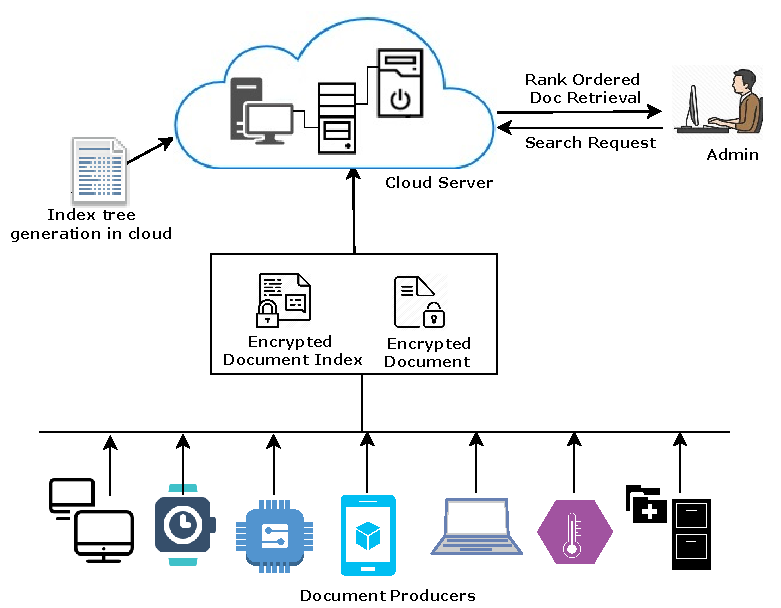
\includegraphics[width=0.97\linewidth]{architechture-thesis}
\caption{RS-PKE Model}
\label{fig:SystemModel}
\end{figure}




\textbf{Document Producers.}
Document producers are lightweight and independent (added/removed dynamically) devices like IoT or smartphones that generate continuous collection of documents $F$ = $\{f_1, f_2, f_3,\dots\}$, to be securely outsourced to cloud. These documents can be mobile application logs, IoT devices' sensor information, or health organizations' medical reports. Encrypted document indexes are created from these documents using the public key, outsourced to the cloud with encrypted documents. The documents can be deleted once they are uploaded to the cloud. 

\textbf{Cloud Server.}
The cloud server stores the encrypted documents and constructs a dynamic, searchable KBB tree-based index from the encrypted document indexes.\looseness=-1

\textbf{Admin.}
The admin initiates the search and has the private key. He has reasonable bandwidth, CPU, and stable connectivity with the cloud. He collaborates with the cloud to perform a keyword-based single or top-k ranked search using the private key.\looseness=-1



Formally, \textbf{RS-PKE} is defined by the following algorithms:

 {\textbf{\texttt{Setup($\lambda$)}:}} takes security parameter $\lambda$ as input and outputs the necessary system parameters $\mathcal{P}$. Admin executes it at beginning. 
    
    
 {\textbf{\texttt{KeyGen($\mathcal{P}$)}:}} takes system parameters $\mathcal{P}$ as input and outputs public-private key pair \texttt{(PubKey, PrvKey)}. Admin distributes the public key to document producers and keep private key for search.
    
 {\textbf{\texttt{{GenDocIndex(f, PubKey}):}}} Document producer take document $f$ and public key \texttt{PubKey} and outputs encrypted document index. This executes for each document to construct document index.\looseness=-1
    
    
{\textbf{\texttt{BuildIndexTree(docIndex, Tree}):}} The cloud takes encrypted document index \texttt{docIndex} and existing index tree \texttt{Tree} as input and then insert \texttt{docIndex} to \texttt{Tree}.
    
{\textbf{\texttt{Search(keyword, k, PrvKey, Tree}):}} takes search keyword \texttt{keyword}, private key \texttt{PrvKey}, and index tree \texttt{Tree} as input. It is a two party algorithm, consists of \texttt{searchAdmin(keyword, k, PrvKey)} and \texttt{searchCloud(Tree)}. It outputs top-k documents (documents with highest TF score) from the \texttt{Tree}. The cloud runs ${BuildIndexTree}$ and ${searchCloud}$, and the admin runs ${searchAdmin}$.



\subsection{Security Model}\label{security-model}



The document producers and the admin in our proposed scheme are trusted entities, except the cloud server. The cloud is termed as ``\textit{honest, but curious}'' in our proposed model. Cloud honestly executes every assigned task; meanwhile, it is curious about the encrypted documents and search keywords. The leakages of RS-PKE can be defined as $\mathcal{L}_{RS-PKE} = (\mathcal{L}_{Setup}, \mathcal{L}_{BuildIndexTree}, \mathcal{L}_{Search})$. The details of the leakages are discussed in section~\ref{leakage}. Formally, we define the following security models for RS-PKE. The security models also imply security guarantees against the outside adversaries, which have fewer capabilities than the cloud.\looseness=-1





\subsubsection{Security of Document Index and Index-Tree}

%The document producers encrypt the document indexes and only the admin has private key to decrypt them. The Cloud has only access to encrypted document indexes. An adversary in the cloud may try to infer document related information. Our security definition of document index follows the security notions of Boneh et al.\cite{boneh2004public}, Curtmola et al.\cite{curtmola2006} and Chen et al.\cite{chen2015new} but we replace \textit{trapdoors} with \textit{keyword search procedure} and \textit{ciphertexts} with \textit{document indexes}. It guarantees that no adversary can distinguish a document index from another one. That is, the document index does not reveal any information about the underlying keywords to any adversary. We introduce a game, namely indistinguishability under adaptive chosen keyword attack (IND-SPKE-CKA), to capture the security of document index. The security game for IND-SPKE-CKA is defined as,\looseness=-1

 An adversary in the cloud may try to infer document related information from the index tree. The index tree is constructed from the document indexes. The security of the index tree depends on the document indexes. We introduce a game, namely indistinguishability under adaptive chosen keyword attack (IND-SPKE-CKA), to capture the security of document index. Our security definition of document index follows the security notions of Boneh et al.\cite{boneh2004public}, Curtmola et al.\cite{curtmola2006} and Chen et al.\cite{chen2015new} but we replace \textit{trapdoors} with {\texttt{Search(keyword, k, PrvKey, Tree}):} and \textit{ciphertexts} with \textit{document indexes}. It guarantees that no adversary can distinguish a document index from another one. That is, the document index does not reveal any information about the underlying keywords to any adversary.  The security game for IND-SPKE-CKA is defined as,\looseness=-1




\begin{definition}\label{ind-spke-cka-game}
IND-SPKE-CKA is an interactive game between an adversary $\mathcal{A}$ and Challenger $\mathcal{C}$ as follows:

\textbf{\textit{Setup}}. $\mathcal{C}$ runs the $KeyGen(\mathcal{P})$ algorithm and gives the $PubKey$ to $\mathcal{A}$. $\mathcal{A}$ has full control over the index tree. That is $\mathcal{A}$ can insert/delete any $docIndex$ in the tree.

\textbf{\textit{Test query-1}}. $\mathcal{A}$ can adaptively request the $docIndex$ of any document $f_i$ or initiate and retrieve top $k$ search results for any keyword $w$ of it's choice from $\mathcal{C}$.

\textbf{\textit{Challenge}}. $\mathcal{A}$ sends $\mathcal{C}$ two documents $f_0$ and $f_1$ of its choice which it wishes to be challenged. $\mathcal{C}$ picks $b\leftarrow\{0,1\}$ and generates,

\begin{equation}
docIndex_b\leftarrow genDocIndex(f_b, PubKey)
\end{equation}

$\mathcal{C}$ sends $docIndex_b$ to $\mathcal{A}$.


\textbf{\textit{Test query-2}}. $\mathcal{A}$ can perform additional computations in polynomial time.

\textbf{\textit{Output}}. $\mathcal{A}$ outputs guess $b'\in \{0,1\}$, if $b' = b$ or in other words if $\mathcal{A}$ can correctly guess whether it was given the document index of $f_0$ or $f_1$, $\mathcal{A}$ wins the game. The advantage that $\mathcal{A}$ wins the game is defined as $Adv_{\mathcal{A}}^{\textit{IND-SPKE-CKA}}= Pr[b' = b]-\frac{1}{2}$.


\end{definition}


\subsubsection{Security of Search Keyword} 



We introduce a security game for the search keyword's security, namely indistinguishability under the chosen search keyword attack for SPKE (IND-SPKE-CSKA). It guarantees that the adversary can not identify search keywords even if they are repeated. We define the security game for IND-SPKE-CSKA as,





\begin{definition}\label{IND-SPKE-CSKA-game}
 IND-SPKE-CSKA is an interactive game between an adversary $\mathcal{A}$ and Challenger $\mathcal{C}$ as follows:

\textbf{\textit{Setup}}. $\mathcal{C}$ runs the $KeyGen(\mathcal{P})$ algorithm and gives the $PubKey$ to $\mathcal{A}$. $\mathcal{A}$ has read-only access to the KBB tree. That is $\mathcal{A}$ can observe insert/delete/search process in the tree.

\textbf{\textit{Test query-1}}. $\mathcal{A}$ can adaptively request the $docIndex$ of any document $f_i$ or initiate and retrieve search results for any keyword $w$ of it's choice from $\mathcal{C}$.

\textbf{\textit{Challenge}}. $\mathcal{A}$ sends $\mathcal{C}$ two keywords $w_0$ and $w_1$ of its choice which it wishes to be challenged and which have not been searched before. $\mathcal{C}$ picks $b\leftarrow\{0,1\}$. $\mathcal{C}$ initiates search for $w_b$ and send the search result (document index) $docIndex_b$ to $\mathcal{A}$.

\textbf{\textit{Test query-2}}. $\mathcal{A}$ can perform additional computations in polynomial time.  

\textbf{\textit{Output}}. $\mathcal{A}$ outputs guess $b'\in \{0,1\}$, if $b' = b$ or in other words if $\mathcal{A}$ can correctly guess whether it was given the search results for $w_0$ or $w_1$, $\mathcal{A}$ wins the game. The advantage that $\mathcal{A}$ wins the game is defined as $Adv_{\mathcal{A}}^{IND-SPKE-CSKA}= Pr[b' = b]-\frac{1}{2}$.

\end{definition}



\subsubsection{Forward Privacy}\label{theorem4}   

Forward privacy ensures the previous search leakages cannot be exploited to infer information about the newly added documents \cite{stefanov2014practical}. In our scheme, the update operation is defined as deletion of the old document from the cloud and adding the updated document (details in \ref{kbb-construction}). Therefore, we will only discuss the Forward Privacy of adding a document. Formally, we define the forward privacy game FS-SPKE of our scheme as,


\begin{definition}\label{fs-game}
 FS-SPKE is an interactive game between an adversary $\mathcal{A}$ and Challenger $\mathcal{C}$ as follows:

\textbf{\textit{Setup}}. $\mathcal{C}$ runs the $KeyGen(\mathcal{P})$ algorithm. $\mathcal{A}$ chooses two keywords $w_0$ and $w_1$ from the dictionary.

\textbf{\textit{Test query-1}}. $\mathcal{A}$ can adaptively initiate and retrieve top $k$ search results for any keyword $w$ of it's choice including $w_0$ and $w_1$ from $\mathcal{C}$.

\textbf{\textit{Challenge}}. $\mathcal{C}$ picks $b\leftarrow\{0,1\}$, adds $w_b$ to a document $f_b$ and generates,

\begin{equation}
docIndex_b\leftarrow genDocIndex(f_b, PubKey)
\end{equation}

$\mathcal{C}$ sends $docIndex_b$ to $\mathcal{A}$.


\textbf{\textit{Test query-2}}. $\mathcal{A}$ can perform additional computations in polynomial time.



\textbf{\textit{Output}}. $\mathcal{A}$ outputs guess $b'\in \{0,1\}$, if $b' = b$, $\mathcal{A}$ wins the game. The advantage that $\mathcal{A}$ wins the game is defined as $Adv_{\mathcal{A}}^{FS-SPKE}= Pr[b' = b]-\frac{1}{2}$.


\end{definition}







\section{Preliminaries}\label{preli}

\subsection{Encryption Technique} \label{encryp_tech}



\textit{Homomorphic encryption (HE)} is a form of encryption that allows any data to remain encrypted while being processed and generates a result in encrypted form, which matches the result of the operations as if they were performed on the plaintext \cite{rivest1978data, acar2018survey}. \textbf{Fully Homomorphic Encryption (FHE)} is still not practical to use in today's big data world as it is impractically slow. It uses complex and computationally heavy operations. Therefore, we propose to use \textbf{Partially Homomorphic Encryption (PHE)}, which supports only a single operation, which in our case, is addition, an unlimited number of times. Our scheme is oblivious to the \textit{PHE} chosen, as long as it supports the following features:\looseness=-1


% It can be categorized into three types of schemes \cite{acar2018survey}. (1) \textbf{Fully Homomorphic Encryption (FHE)}: it supports unlimited number of arbitrary functions (e.g., searching, sorting, max, min, etc.), unlimited number of times. Example : Helib, libScarab, Microsoft SEAL. (2) \textbf{Somewhat Homomorphic Encryption (SwHE)}: It supports all types (a logically complete set) of operations (e.g., addition and multiplication) but a limited number of times (e.g., limited circuit depth). Example: Sande-Tomas-Young, Boneh-Goh-Nissim, Ishai-Yuval-Paskin. (3) \textbf{Partially Homomorphic Encryption (PHE)}: It supports one type of operation, unlimited number of times. Example: Goldwasser-Micali Cryptosystem, Okamoto-Uchiyama Cryptosystem, Paillier Cryptosystem, El-Gamal Cryptosystem.
 
 






{\textbf{Public-Key Encryption}}: The encryption is an asymmetric key PHE, consists of a public-private key pair ($PubKey$, $PrvKey$). Distributed document producers have the risk of key leakage. Therefore symmetric key encryption is not suitable.
    
{\textbf{Additive and Subtractive Homomorphism}}: The encryption supports an addition operator $\boxplus$ and a subtraction operator $\boxminus$ such that for $Enc(a,$ $PubKey)$ $\xrightarrow{}$  $e_a$ and $Enc(b,$ $PubKey)$ $\xrightarrow{}$ $e_b$, $Dec(e_a$ $\boxplus$ $e_b,$ $PrvKey)$ $\xrightarrow{}$ $a$ $+$ $b$ and $Dec(e_a \boxminus e_b, PrvKey) \xrightarrow{} a-b$. Subtraction is used for optimization, however this is an optional feature. 
    
{\textbf{Indistinguishability under Chosen Ciphertext Attack (IND-CCA1)}}: We assume the PHE scheme is IND-CCA1 secure, which is the highest security level for HE (due to their malleability). Though general IND-CCA1 security of PHE is an open question, many PHE like Paillier cryptosystem has proven to be IND-CCA1 secure \cite{lipmaa2010cca1, armknecht2013group}. Although, an Indistinguishability under Chosen Plaintext Attack (IND-CPA) secure PHE can also work in RS-PKE with fewer security guarantees by modifying Definition~\ref{ind-spke-cka-game} and~\ref{IND-SPKE-CSKA-game}. The security game of IND-CCA1 is given in Appendix~\ref{ind-cca1}.\looseness=-1
    
    
 

\subsection{Notations}
\begin{itemize}
\item[$-$] $\boldsymbol{F}$, The  plain text document collections, $\boldsymbol{F} = \{f_1, f_2, f_3, f_4\dots\}$.

\item[$-$] $\boldsymbol{W}$, The dictionary is the unique set of keywords used in search, $\boldsymbol{W} = \{w_1, w_2, w_3,\dots,w_N\}$.

\item[$-$] $\boldsymbol{N}=|\boldsymbol{W}|$ is the number of words in $\boldsymbol{W}$.
\end{itemize}

% \subsection{Vector Space Model Construction}
% Vector space model with \textit{term frequency-inverse document frequency (TF-IDF)}, is a numerical statistic that indicates how important or relevant a word is to a document in a collection of documents\cite{ullman_2011}. There are many variations of the \textit{TF-IDF} weighting scheme. We have used the definition from \cite{ullman_2011} in our scheme. \textit{Term Frequency (TF)} indicates the weight of a keyword in a document. Suppose we have a collection of $N$ documents, $FR_{ij}$ is the frequency of keyword $w_i \in W$ in document $f_j$ and $\max_k FR_{kj}$ is the maximum frequency of any keyword $w_k \in W$ in document $f_j$. Then, ${TF_{ij}}$, is defined as: $    TF_{ij} = \frac{FR_{ij}}{\max_k FR_{kj}}$.


% In our scheme, we normalized the TF scores by multiplying it with a constant value of $\alpha$ and rounding it to the nearest integer. $\alpha$ is the normalization factor, which is combined with rounding function $\lfloor \rceil$ to make the TF based relevance score an integer in $[0-\alpha]$ range. 

%  \textit{Inverse Document Frequency} $IDF$ indicates how important a word is in a document collection or how much information the word provides. In the future, we plan to extend our framework to support a multi-keyword ranked search using the \textit{TF-IDF} model with pre-computed $IDF$ \cite{xia2015secure}.


\subsection{Keyword Balanced Binary Tree (KBB tree) Construction}


% The keyword balanced binary (KBB) tree in our scheme is a
% dynamic data structure whose node stores a vector D. The
% elements of vector D are the normalized TF values. Sometimes, we refer the vector D in the node u to Du for simplicity. Formally, the node u in our KBB tree is defined as
% follows:


KBB tree \cite{xia2015secure} is a dynamic balanced binary tree where each node \texttt{Node} can be defined as:
\begin{center} 
{\texttt{
 Node $\leftarrow$ $\langle$ ID, Data, Left, Right, Parent $\rangle$}
}
\end{center}
where, 
\newline\texttt{ID} denotes unique identifier for each tree node,
\newline\texttt{Data} is a vector with length $N$ (size of the keyword dictionary),
\newline\texttt{Left}, \texttt{Right} and \texttt{Parent} indicate the left, right, and parent node. 

In the leaf level, node \texttt{LeafNode} denotes a specific document $f$ and \texttt{LeafNode.Data[i]} stores the normalized TF score of keyword $w_i$ in $f$. For internal node \texttt{InternalNode},
\newline\texttt{
    InternalNode.Data[i] $\xleftarrow{}$ max(InternalNode.Left.Data[i], InternalNode.Right.Data[i]), i= 1, $\dots$, N
    }



The owner can perform multi keyword ranked search in Xia et al.'s scheme. The owner first creates a vector $trapdoor$ for the searched keywords and sends it to the cloud. The relevance score $RScore$ of any node for that query in the index tree is calculated using $RScore \xleftarrow{} Data \cdot trapdoor$. The cloud then performs a recursive procedure upon the tree, named as “Greedy Depth-first Search” (GDFS). The cloud uses $RScore$  to greedily select which nodes are accessed during GDFS and return the top-k documents with the largest relevance scores for that query to the owner. 

However, with this approach, the cloud can store the $trapdoor$ and use it extensively without the owner's knowledge. The relevance scores are leaked to the cloud, which might be used in leakage abuse attacks. If the document collection in owner side updated, the KBB tree in the cloud also need to be updated. In order to
reduce the communication overhead, the data owner
stores a copy of unencrypted index tree. The owner modifies the KBB tree in his end and send updates it to the cloud.


\section{RS-PKE Construction}\label{proposed}




In this paper, we develop a secure SPKE search framework over encrypted cloud data that allows the cloud server to perform a ranked keyword search without knowing the document producer's sensitive information. As stated earlier, the proposed scheme consists of three entities: document producer, cloud server, and admin. Each entity plays a different role in the data outsourcing environment. The document producer encrypts the document and creates an encrypted document index. Both of them are outsourced to the cloud. The cloud then generates an encrypted dynamic KBB tree-based index from the encrypted document indexes according to the techniques discussed in \ref{kbb}. Our novel approach uses a partially homomorphic encrypted KBB tree-based index to mitigate the security concerns raised by a ``\textit{honest, but curious}'' cloud server. An admin can initiate a search request for a specific keyword and retrieve the best matched (highest $TF$ score) documents through an interactive search protocol. 

\subsection{Proposed Modified KBB Tree}\label{kbb}

\begin{figure}[htb]
    \centering
    \subfloat[]{
       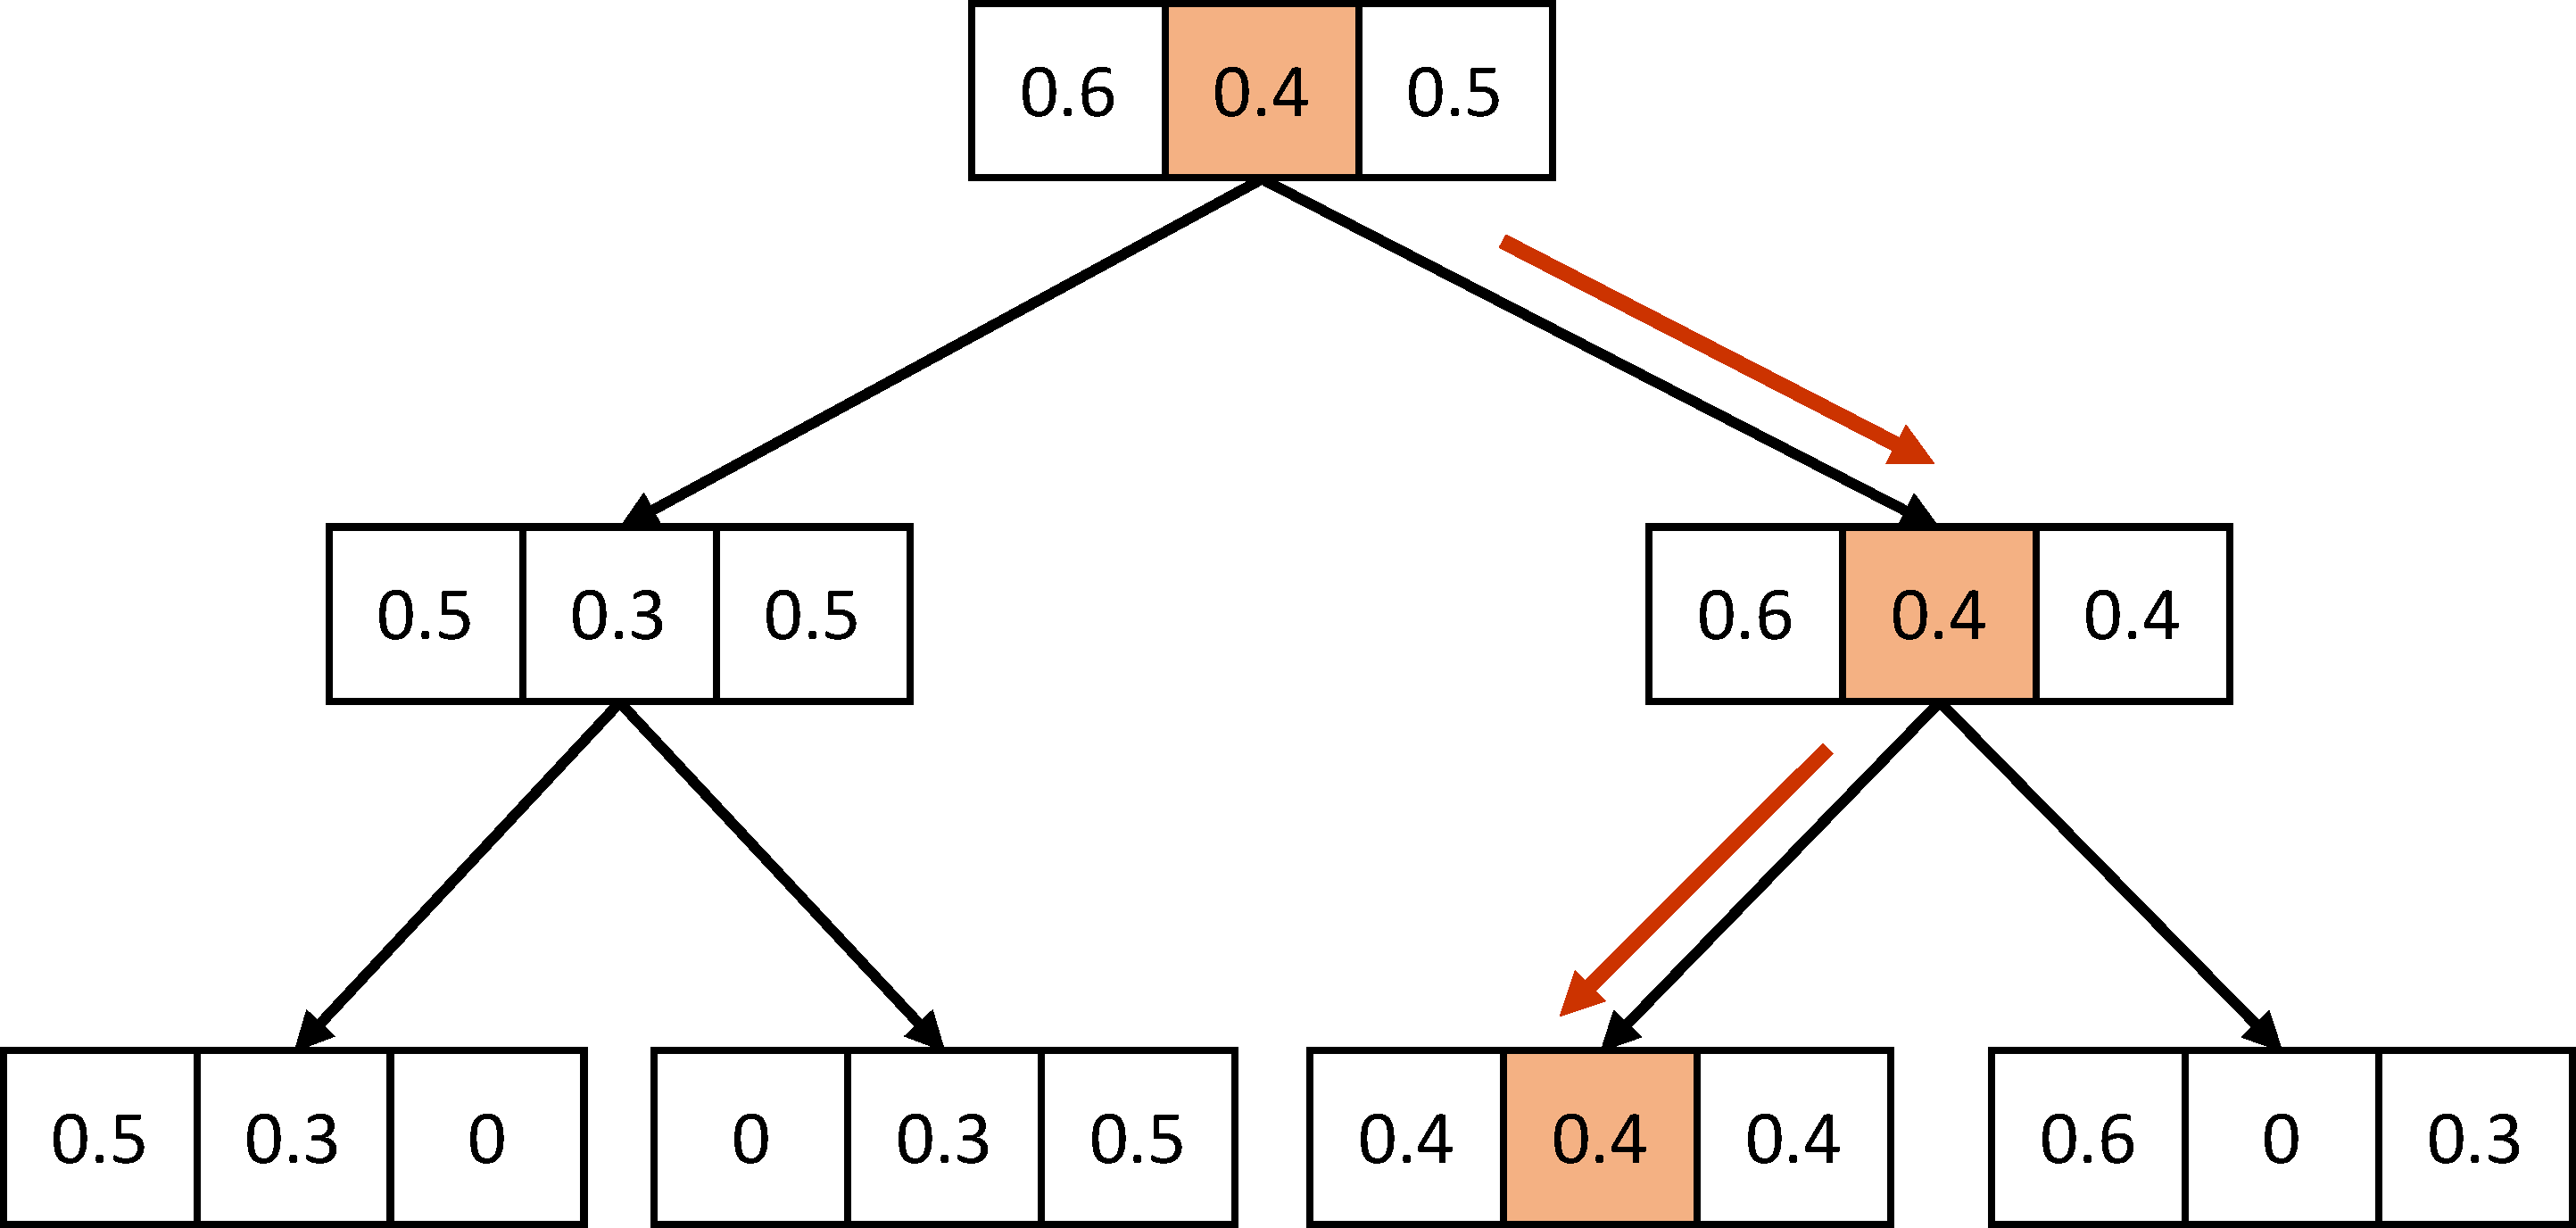
\includegraphics[width=0.85\linewidth]{Orig_KBB.pdf}}
       \hfill
  \subfloat[]{
        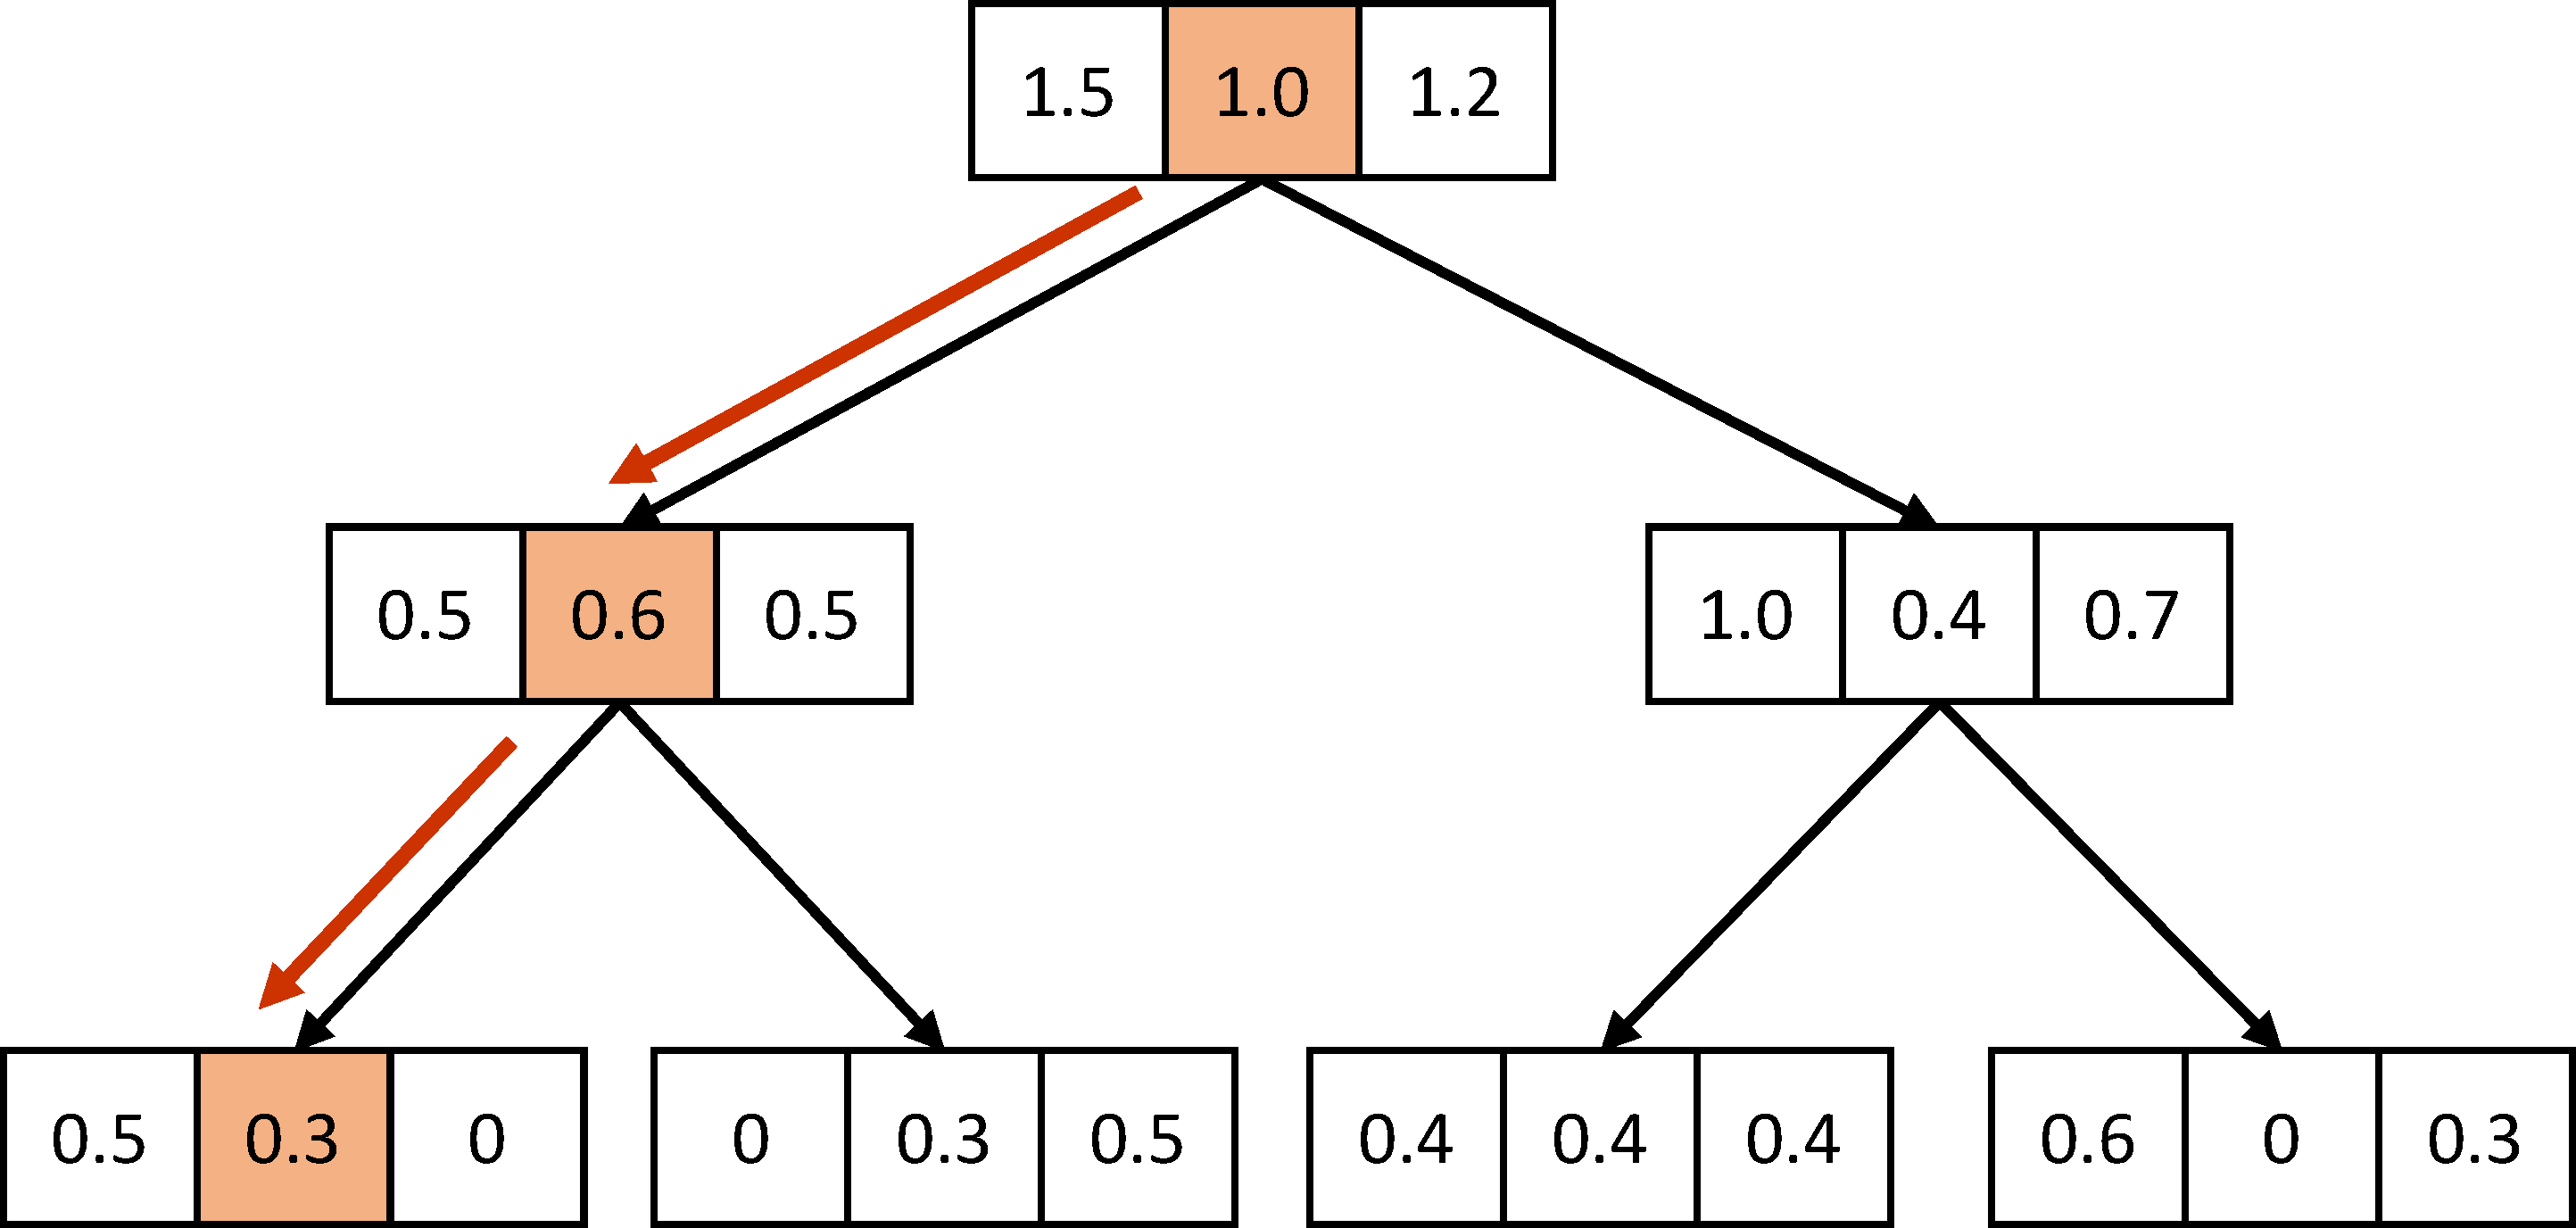
\includegraphics[width=0.85\linewidth]{Wrong_KBB.pdf}}
        \hfill
  \subfloat[]{
        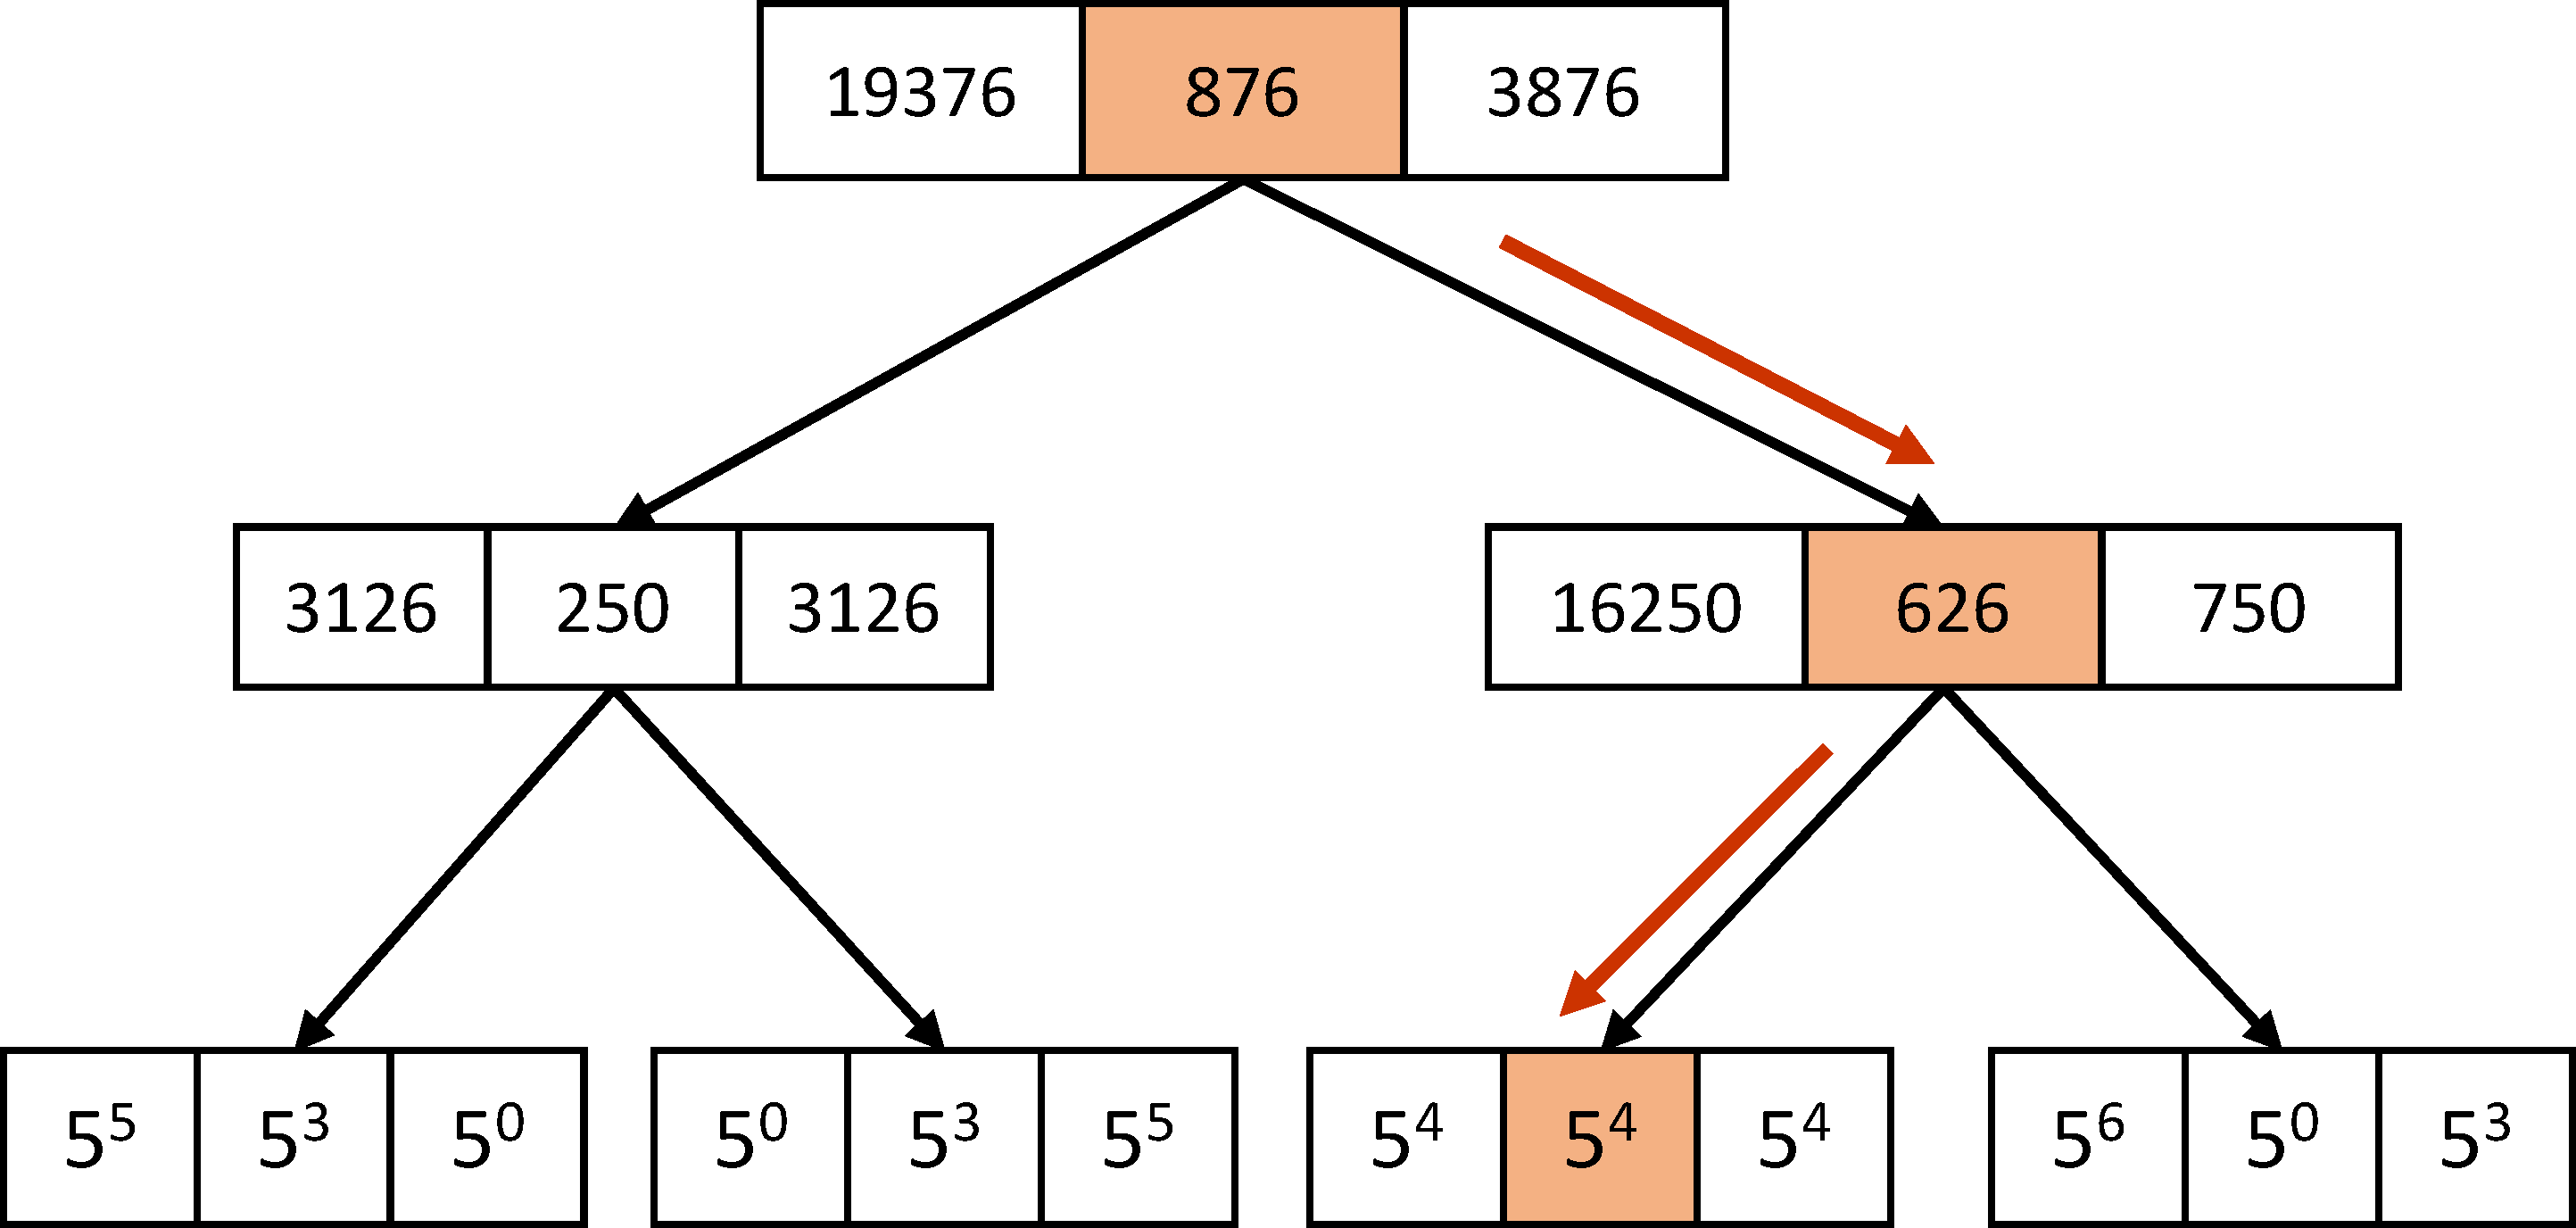
\includegraphics[width=0.85\linewidth]{Our_KBB.pdf}}
  \caption{\small{An example of the KBB tree-based indexes with 4 documents, the cardinality of the dictionary is 3, and search is for the topmost relevant document for the second word. In all cases, the search starts at the root node and reaches the leaf node by following the node's path with the maximum value. Figure (a) is the original KBB tree, where leaf nodes represent documents and the internal nodes are generated by taking the \textit{maximum} value between the child nodes. This tree is generated at owner side on plaintext data. Figure (b) is the same tree; however, we used \textit{addition} operation to generate the internal nodes instead of \textit{maximum} operation. As our proposed tree is generated dynamically on cloud and we need to operate on encrypted data, we cannot do \textit{maximum} operation. However, \textit{addition} cannot preserve the relative ordering between nodes required for searching. In figure (c), the data values of the leaf nodes are applied to function $b()$ with $\alpha = 10$ and $M = 5$, and then the internal nodes are constructed like figure (b). Theorem~\ref{b-theorem} enables us to use the same searching mechanism as the original KBB tree by preserving relative ordering through homomorphic addition.\looseness=-1}}
\label{fig:treeWithB} 
\end{figure}
%   
  
  

  
  
  
%   In the construction process of the tree index, we first generate leaf nodes from the documents. Then, the internal tree nodes are generated based on the leaf nodes. This figure also shows an example of search process.  with size of the dictionary $N=1$. In (b) each leaf node's value is the encrypted normalized $TF$ score applied to $b()$. The minimum value of $M$ is 5 as the value of $D_{max}$ in this example is 8. These figures show an example of the search process, in which the query vector $Q$ searches for the document with maximum normalized $TF$ score.Fig. \ref{fig:treeWithB} depicts our searching in the proposed KBB tree with only single keyword ($N = 1$) for searching the most relevant document ($k = 1$). In Fig. \ref{fig:treeWithB}(a), we have shown a simple KBB tree without encoding. In Fig. \ref{fig:treeWithB}(b), the relevance scores are encoded using $b()$. 

The KBB tree of RS-PKE is based on Xia et al.'s KBB tree. Our node and tree structures are similar to Xia et al. However, our design goals are different. For supporting lightweight platforms like IoT: (1) The value of the nodes should be encrypted using the public key and decrypted using the private key,
(2) The lightweight document producers should not store the unencrypted index tree as the owner does in Xia et al, and
(3) The encrypted document index generation for a specific document in the document producers' side should be faster and should not require any information about the existing tree like Xia et al. The document producer should be able to generate encrypted documents and document index, upload, and delete them without keeping any information. Xia et al. focused on faster initial tree generation and search, where we focused on a faster dynamic update of documents. In addition, we wanted to make RS-PKE forward secure and not leak relevance scores to the cloud.\looseness=-1


We found out that partial homomorphic encryption can be used to encrypt document indexes (normalized $TF$ values), and the cloud can operate on encrypted document indexes to generate the KBB tree. This encrypted document index is stored in \texttt{Data} vector of the leaf nodes. The internal nodes are generated by the homomorphic addition of the left and the right child nodes.\looseness=-1
\newline$InternalNode.Data[i] \xleftarrow{}$\\ $InternalNode.Left.Data[i] \boxplus InternalNode.Right.Data[i]$,\\
    $i= 1, \dots, N$
    

We cannot take \textit{maximum} of left and right child nodes to generate the internal node like the original KBB tree as we are operating on partially homomorphically encrypted data in the cloud. Doing \textit{maximum} operation on encrypted data would require the document indexes to be encrypted using FHE which is vey slow. The \textit{maximum} operation was possible in Xia et al.'s scheme as the KBB tree was generated on the owner side on plaintext data.  

However, this internal node construction process nullifies relative order information between nodes which is required during searching (example in Fig.~\ref{fig:treeWithB}(b)). To preserve the relative ordering thorough addition, it must be ensured that if the leaf node with the highest relevance score resides in the right subtree, the summation of relevance scores in the right subtree must be larger than the summation of all leaves of the left subtree.
For this, we exploit the fact that, if $max(a, b) > max(c, d)$ then for a sufficiently large $M$,

\begin{equation*} 
\begin{split}
M^a + M^b >{}& M^{max(a, b)}
\geq M^{max(c, d) + 1} = M . M^{max(c, d)}
> 2 . M^{max(c, d)}\\
>{}& M^c + M^d
\end{split}
\end{equation*}

Using this, we define a function $b()$: $\mathbb{N}_0\xrightarrow{}\mathbb{N}_0$ to preserve relative order through the sum.

\begin{theorem}\label{b-theorem}
If the function $b()$ can be defined as:
 \begin{equation} 
\label{eq3_1}
\begin{split}
 b(s)  &= M^s
 \end{split}
\end{equation}

Where, 

\begin{itemize}
    \item[$-$] $s$ is the normalized $TF$ based relevance score
    
    \item[$-$] $M$ $=$ $\lfloor\frac{D_{max}}{2}\rfloor+1$ , where $D_{max}$ is the maximum number of documents the system can handle. This proof assumes that, $D_{max} > 1$
\end{itemize}


then, the function $b()$ has the following properties:
    \begin{itemize}
         \item[$-$] $b(0)$ is the smallest output of $b$
          \item[$-$] $b(s_{max}) > \sum b(j)$, here, $s_{max}$ is the maximum relevance score in the tree and $j \in$ all relevance scores of the subtree where $s_{max}$ does not reside.
    \end{itemize}

\end{theorem}

The proof of Theorem~\ref{b-theorem} is given in Appendix~\ref{b-proof}. The transformed relevance scores are encrypted to create document indexes (details in \ref{docindex}) and the KBB tree is constructed in cloud using partial homomorphic addition (details in  \ref{kbb-construction}). The two properties of $b()$ ensure that the search procedures described in \ref{kbb-searching} give correct results (example in Fig.~\ref{fig:treeWithB}(c)).






 
% \begin{figure}
%     \centering
%     \subfloat[]{
%       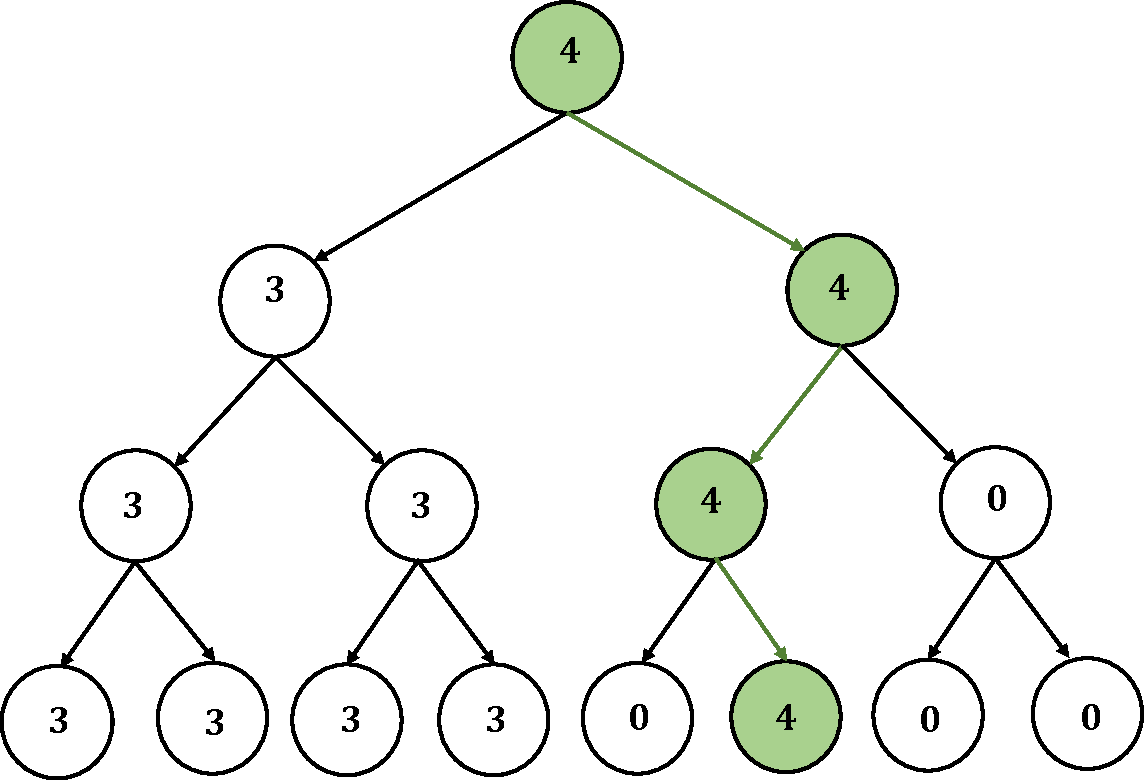
\includegraphics[width=0.7\linewidth]{pdfs/binarySearchTree.pdf}}
%     \hfill
%   \subfloat[]{
%         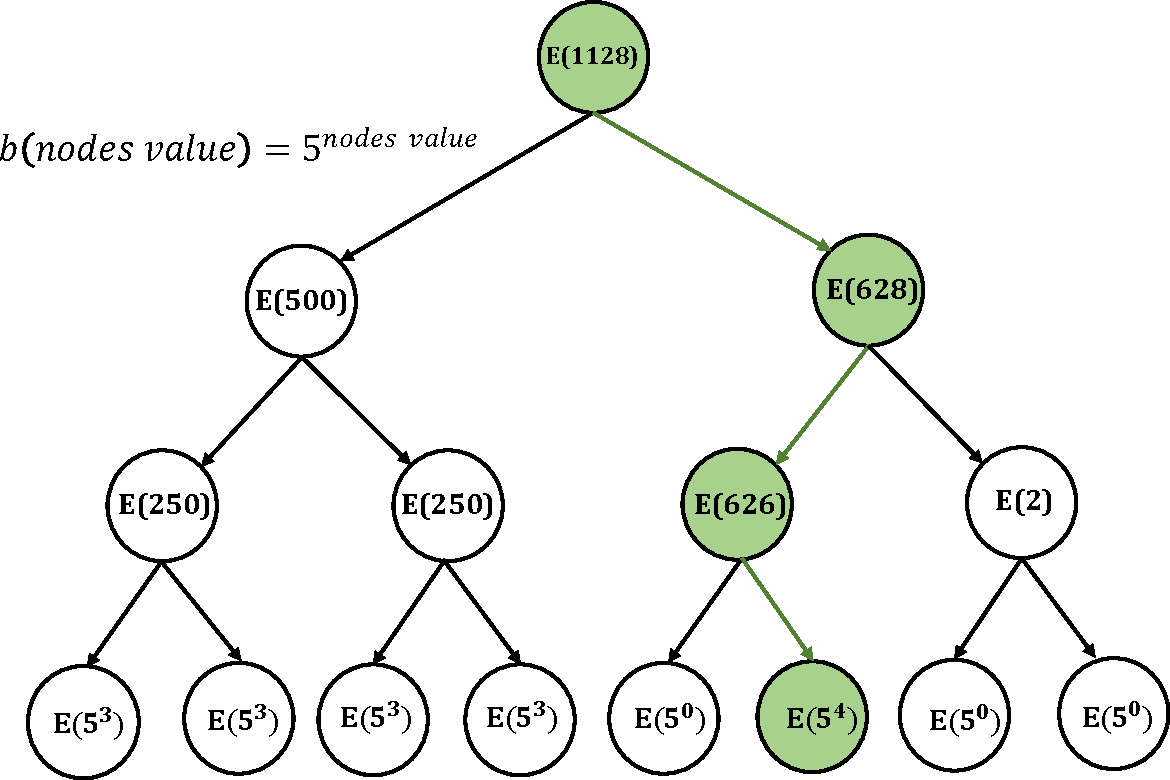
\includegraphics[width=0.7\linewidth]{pdfs/treeWithB().pdf}}
%   \caption{Comparison of (a) original KBB tree and (b) our proposed KBB tree with size of the dictionary $N=1$. In (b) each leaf node's value is the encrypted normalized $TF$ score applied to $b()$. The minimum value of $M$ is 5 as the value of $D_{max}$ in this example is 8. These figures show an example of the search process, in which the query vector $Q$ searches for the document with maximum normalized $TF$ score.\looseness=-1 }
%   \label{fig:treeWithB} 
% \end{figure}






\subsection{System Description}

\subsubsection{\textbf{Setup}}

$Setup()$ takes security parameter $\lambda$ as input and outputs dictionary $W$ with cardinality $N$, normalized factor $\alpha$, the maximum number of documents the system can support $D_{max}$, and $M$. Though our system supports dynamic document addition functionality, yet a fixed dictionary $W$ is used. Realistically, in IoT, mobile, or healthcare systems, the keyword space usually doesn't change much. Therefore, an adequately sized fixed dictionary will suffice. The dictionary can also be updated later to accommodate more keywords by doing a $Setup()$ and migration but without changing public-private key pair. Care must be taken while choosing the value of $\alpha$ as a small value can cause unequal frequencies being tied. Thus potentially inaccurate results to a top-k query and large value can cause the system performance to hamper. Similarly, smaller $M$ can introduce error in search, but larger $M$ hampers performance. Though theoretically minimum value of $M =\lfloor\frac{D_{max}}{2}\rfloor+1$ is needed, in a real dataset, keywords are more distributed, and hence values much less than the minimum $M$ would work accurately.





\subsubsection{\textbf{Keygen}}

    
$Keygen()$ takes system parameters as input and outputs public-private key pair ($PubKey$, $PrvKey$) for the underlying partial homomorphic encryption. The keys are distributed to document producers and the admin, respectively.




\subsubsection{\textbf{Encrypted Document and Document Index Generation}}\label{docindex}

Documents produced by the document producers can be encrypted using any standard file encryption technique. Therefore, the encryption process of documents is not the primary concern of this paper. Our proposed scheme mainly focuses on the construction of encrypted document index. For measuring the relevance of a document to a keyword, we are using \textit{Term Frequency (TF)}, which indicates the weight of a keyword in a document. Formally, the encrypted document index of a document $f$, is constructed using the following equation:

\begin{equation}
\begin{split}
    E=Enc(b(\lfloor \alpha * TF_{1} \rceil), PubKey), Enc(b(\lfloor \alpha * TF_{2} \rceil), PubKey),\\
    Enc(b(\lfloor \alpha * TF_{3} \rceil), PubKey),\dots, Enc(b(\lfloor \alpha * TF_{N} \rceil), PubKey)
\end{split}
 \end{equation}

Here, $TF_{i}, i \in [1-N]$ denotes TF score of $i^{th}$ word in the dictionary for $f$. ${TF_{i}}$, is defined as: $TF_{i} = \frac{FR_{i}}{\max_k FR_{k}}$. Here, $FR_{i}$ is the frequency of each keyword $w_i \in W$ and $\max_k FR_{k}$ is the maximum frequency of any keyword $w_k \in W$ in document $f$. The $TF$ score is then normalized by multiplying with $\alpha$ and rounded to an integer in $[0-\alpha]$ range to be applied to function $b()$ of equation \ref{eq3_1}. The output of function $b()$ is then encrypt using the $PubKey$.


 
% Fig. \ref{fig:encrypteddocumentpolicy} depicts an example of generation of encrypted document index for a document. 
The formal construction process of generating a document index is presented in Algorithm~\ref{encdoc}.


% \begin{figure}[!b]
% 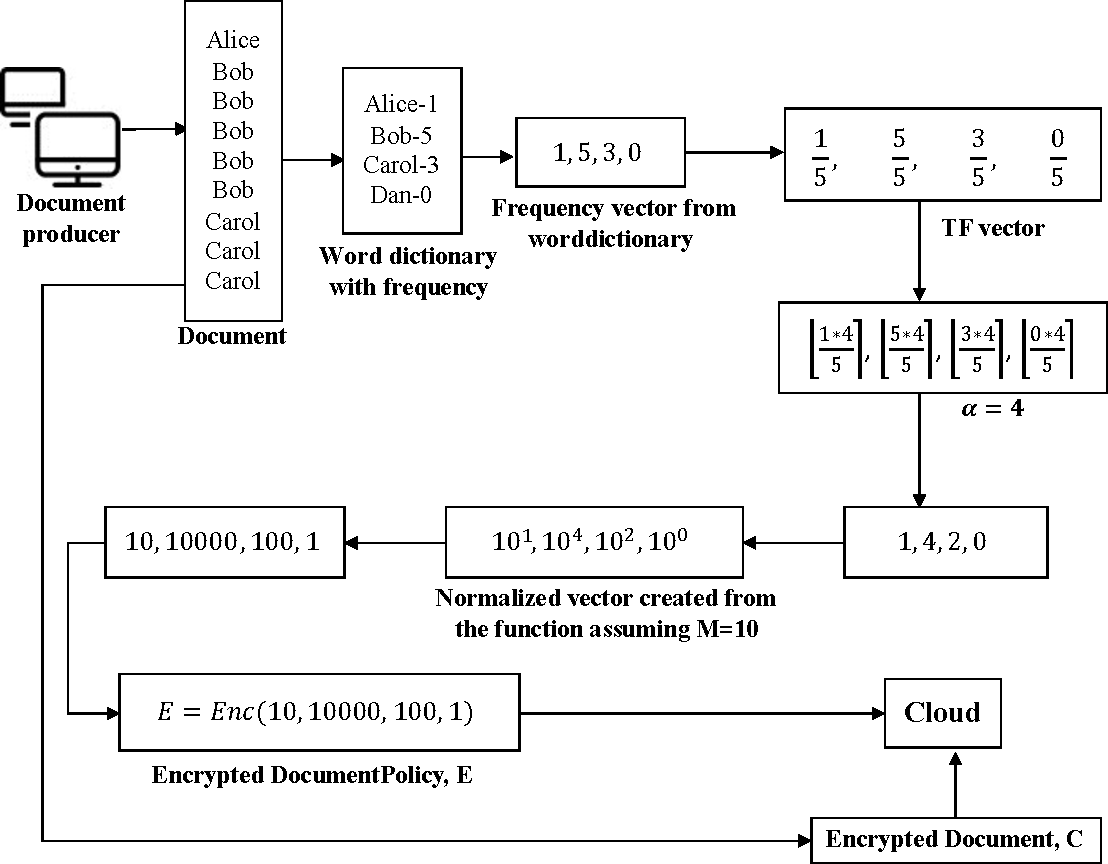
\includegraphics[width=\linewidth]{filepolicy.pdf}
% \caption{An example of the generation of Encrypted document Policy from Documents.}
% \label{fig:encrypteddocumentpolicy}
% \centering
% \end{figure}




\begin{algorithm}[!b]
\small{
\SetAlgoLined
\KwData{Document $f$}
\KwResult{Encrypted $f$ with encrypted document index $E$ to the cloud}
 
 \ForEach{$w \in W$}{
    compute $tf$ for $w$ \;
    $h \xleftarrow{} b(\lfloor \alpha * tf \rceil)$, $e \xleftarrow[]{} Enc(h, PubKey)$\; 
    Insert $e$ to $E$ \;
 }
 Send (Encrypted $f$, $E$) to cloud\;
 \caption{genDocIndex}
 \label{encdoc}
 }
\end{algorithm}



\subsubsection{\textbf{Dynamic KBB Tree Construction}}\label{kbb-construction}

In Section \ref{kbb}, we have briefly introduced our modified version of \textit{KBB} index tree structure. The tree dynamically changes with the insertion or deletion of documents as the leaf node. A tree node can be defined as:
\begin{center} 
{\texttt{
 Node $\leftarrow$ $\langle$ ID, Data, Left, Right, Parent $\rangle$}
}
\end{center}
where, \texttt{ID} denotes unique identifier for each tree node, \texttt{Data} is the encrypted document index for leaf nodes, the homomorphic summation of it's left and right child's data for other nodes. \texttt{Left}, \texttt{Right} and \texttt{Parent} indicates the left, right, and parent node, respectively.


\textbf{Insertion}: A leaf node in the index tree is introduced for each document in the collection with document \texttt{ID} and encrypted document index as the \texttt{Data}. The internal tree nodes are computed by adding it's left child and right child's data values using the addition of PHE. The formal construction process of the index tree is presented in Algorithm~\ref{TreeConstruction}. In Algorithm~\ref{TreeConstruction}, a new document index is inserted in a free leaf node, and the parent nodes are updated accordingly. \texttt{freeNodes} represents all the free leaf nodes. If there are no more free leaf nodes, we increased the tree's height by duplicating the existing tree and merged both trees under a new root.\looseness=-1

% \begin{figure}[!t]
% 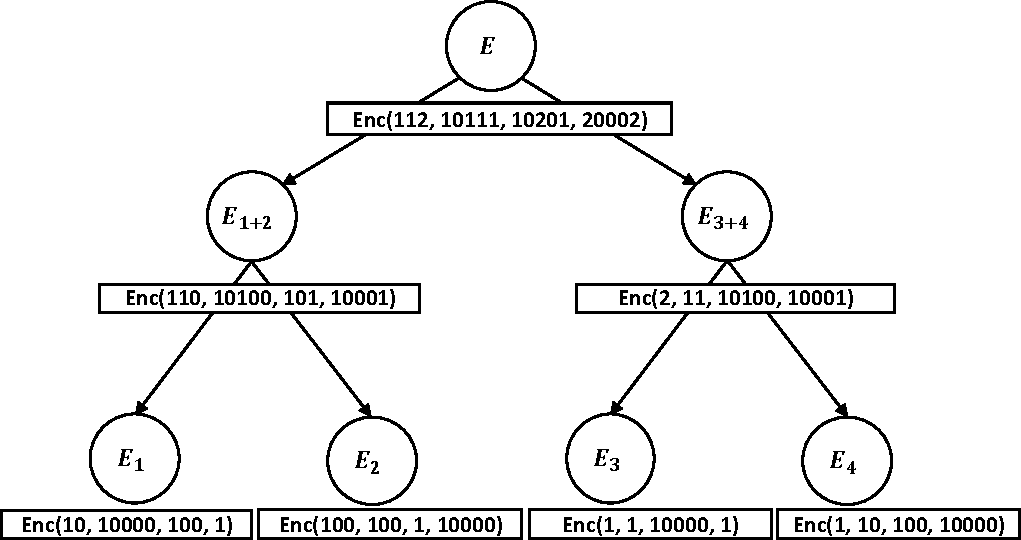
\includegraphics[width=0.95\linewidth]{pdfs/treeInCloud.pdf}
% \caption{\small{An example of the construction process of KBB tree based index. The leaf nodes($E_1$, $E_2$, $E_3$ and $E_4$) represent 4 document indexes and the internal parent nodes are generated by adding the \textit{data} values of leaf nodes. Parent $E_{(1+2)}$ is constructed by homomorphically adding the \textit{data} values of node $E_1$ and $E_2$ nodes. In a similar way $E_{(3+4)}$ and root node $E$ is constructed.}}
% \label{fig:treeInCloud}
% \centering
% \end{figure}


\begin{algorithm}
\small{
\SetAlgoLined
\KwData{encryprted document $c$, doc index $data$}
\KwResult{The Index tree}
    \If{There is no existing tree} {
        Create a new leaf node $u$ with $u.ID \xleftarrow{} GenID()$, $u.left \xleftarrow{} u.right \xleftarrow{} null$ and $u.data \xleftarrow{} null$\;
       Insert $u$ to $freeNodes$, $u$ is the root of the index tree\;
    }
    \ElseIf{$freeNodes$ is empty} {
        \SetKwBlock{Fna}{\textnormal{Create a binary tree $newTree$ of same size as the existing tree}}{}
        \Fna{
            \ForEach{leaf of existing tree} {
               Create a new leaf node $u$ with $u.ID \xleftarrow{} GenID()$, $u.left \xleftarrow{} u.right \xleftarrow{} null$ and $u.data \xleftarrow{} null$\;
               Insert $u$ to $freeNodes$ and $listOfNodes$\;
            }
            \While{$listOfNodes$ has more than 1 node} {
                \While{$listOfNodes$ is not empty} {
                    Take and remove front two nodes $(u,v)$ from $listOfNodes$\;
                    Create a new parent node $p$\;
                    $p.data \xleftarrow{} null$\;
                    $p.left \xleftarrow{} u$, $p.right \xleftarrow{} v$\;
                    $u.parent \xleftarrow{} p$, $v.parent \xleftarrow{} p$\;
                    Insert $p$ to $tempNodeSet$\;
                }
                Replace $listOfNodes$ with $tempNodeSet$ and then clear $tempNodeSet$\;
            }
            
        
        }
        
        Create a new node $newRoot$ with existing tree's root as $newRoot.left$, new tree's root as $newRoot.right$ and existing tree's root's data as $newRoot.data$\;
        Set $newRoot$ as the new root and the combined tree as existing tree.
    }
    Take a free leaf node $u$ from $freeNodes$. Store $c$ with $u.ID$ in the cloud storage. Set $data$ in $u.data$.\;
        \While{$u$ is not $null$} {
            \If{$u.data = null$} {
                $u.data \xleftarrow{} data$\;
            }
            \Else {
                $u.data \xleftarrow{} u.data \boxplus data$\;
            }
            $u \xleftarrow{} u.parent$\;
        }
 \caption{buildIndexTree}
 \label{TreeConstruction}
 }
\end{algorithm}





\textbf{Deletion}: The deletion of a node requires the document producer or the admin to send the document identifier to the cloud, and the cloud deletes the node corresponding to that identifier. After the deletion of a node, the subsequent parent nodes are also updated to adjust the new changes in a similar fashion of data insertion in Algorithm~\ref{TreeConstruction}. The data value of the deleted node gets subtracted from all the subsequent parent nodes. The formal deletion process of a node from the tree is presented in Algorithm~\ref{TreeDelete}.

\begin{algorithm}[!t]
\small{
\SetAlgoLined
\KwData{The id of the document to be deleted, $id$}
\KwResult{The index tree}
        Find the leaf node $node$ associated with $id$\;
        $data \xleftarrow{} node.data$\;
        $parent \xleftarrow{} node.parent$\;
        Remove $node$'s reference from it's $parent$\;
        Delete the document associated with $id$ from cloud\;
        \While{$parent \ne null$} {
            $parent.data \xleftarrow{} parent.data \boxminus data$\;
            $parent \xleftarrow{} parent.parent$\;
        }
        Add $node$ to $freeNodes$\;

\caption{deleteNodeIndexTree}
 \label{TreeDelete}
 }
\end{algorithm}


\textbf{Update}\label{update}: As we have a lightweight document producer so the document is not stored once they are uploaded to cloud. Therefore, one way to update in our system is that first deleting the old document and then reinserting the updated document.


\subsubsection{\textbf{K Ranked Documents Search}}\label{kbb-searching}







% \textbf{Single Document Search}\label{single-search}: In single document searching, at first, a search request for a specific keyword is initiated from the admin. The keyword is kept to the admin. The admin asks the cloud to subtract the value of the right child node from the left child node of the root. The cloud passes the subtraction vector to the admin. The admin then decrypts the value that corresponds to the searched keyword using the private key, and if the decrypted value is \textit{positive}, then the next node to be traversed in the index tree is the \textit{left child node} else the \textit{right child node}. The admin then again repeats the same procedure for the next node. This procedure goes on until the cloud reaches the leaf node. Once the cloud reaches the leaf node, then it sends the \textit{encrypted document} corresponding to that node to the admin. Due to the particular KBB tree-based structure of the index, the number of communication between the admin and cloud is kept to logarithmic. Therefore, this search mechanism involving the admin and the cloud achieves sub-linear search efficiency with some round trip communication.\looseness=-1


 


\begin{algorithm}[htpb]
\small{
\SetAlgoLined
\KwData{$id$ of the node to be traversed from admin}
\KwResult{Subtracted value of child nodes or $null$ if leaf node}


        Find the leaf node $node$ associated with $id$\;
        \If{$node.left= null$ and $node.right= null$} {
            \Return{$null$}\;
        }
        \ElseIf{$node.right.data = null$} {
            \Return{$node.left.data$}
        }
        \ElseIf{$node.left.data = null$} {
            \Return{$node.right.data$}
        }
          \Else {
            \Return{$node.left.data \boxminus node.right.data$}\;
        }
        
    

 \caption{searchCloud}
 \label{algo:searchingInCloud}
 }
\end{algorithm}


% \begin{algorithm}[htpb]
% \small{
% \SetAlgoLined
% \KwData{SearchQuery for the $i^{th}$ word where $w_i \in \boldsymbol{W}$, communication protocol of $tree$}
% \KwResult{Most relevant decrypted document $f$ for $w_i$}
% Get root node's id $id$ from the cloud\;
% \While {$TRUE$} {
%             Let, $difference$ is the output of Algorithm~\ref{algo:searchingInCloud} from the cloud for current node with $id$\;
%             \If{$difference$ is $null$} {
%                 Take encrypted document $c$ with $id$ from the cloud\;
%                 \Return{$decrypt(c)$}\;
%             }
%             $decryptedValue \xleftarrow{} decrypt(difference[i])$\;
%             \If{$decryptedValue \geq 0$}{
%                 Get current node's left child's id from the cloud as $id$\;
%             }
%             \Else{
%                 Get current node's right child's id from the cloud as $id$\;
%             }
%       }
% \caption{searchAdmin}
% \label{algo:searchingInUser}
% }
% \end{algorithm}





\begin{algorithm}[htbp]
\small{
\SetAlgoLined
\KwData{Searching for $k$ documents for the $i^{th}$ word $w_i \in \boldsymbol{W}$, communication protocol with tree as $tree$}
\KwResult{Decrypted $k$ ranked documents for $w_i$}
Get root node's id $id$ and data $data$ from the cloud\;
Decrypt $data$'s $i^{th}$ element and store it in both $value$ and $valueBackup$\;
\BlankLine
\SetKwBlock{Fna}{\textnormal{Convert $value$ into a $M$ base number}}{}
        \Fna{
\While {$value > 0$} {
    Push ($value \mod M$) to stack, $value \xleftarrow{} \lfloor \frac{value}{M} \rfloor$\;
}
Let, $digitSum \xleftarrow{} 0$ \;


\While {$digitSum \leq k$} {
    % pop a value from the stack and add this to $digitSum$\;
    pop from stack to $digitSum$\;
}
}

\BlankLine
Set $minScore$ to $M^{stackSize}$\;
Let, $priorityQueue$ stores the $k$ accessed documents with the largest relevance scores to the query and is always sorted by relevance score in descending order\;
\BlankLine
$dfsRanked(id, valueBackup)$\;
\Return{List of documents whose ids are in $priorityQueue$ by retrieving them from the cloud}\;
\BlankLine


\SetKwFunction{FMain}{dfsRanked}
    \SetKwProg{Fn}{def}{:}{}
    \Fn{\FMain{$id$, $sumChild$}} {
    Let, $difference$ is the output of Algorithm~\ref{algo:searchingInCloud} from the cloud for current node with $id$\;
    
    \If{$difference$ is $null$} {
    
    \If{$priorityQueue$ has fewer elements than $k$}{
                Insert ($id$, $sumChild$) to $priorityQueue$\;
            }
    \Else{
    \If{$sumChild$ is greater than smallest element of $priorityQueue$}
    {Delete the element with smallest relevance score from $priorityQueue$\;
    Insert ($id$, $sumChild$) to $priorityQueue$\;
    }
            }
        }
    \Else{
        $subChild \xleftarrow{} decrypt(difference[i])$\;
        $leftChild \xleftarrow{} \frac{sumChild + subChild}{2}$, $rightChild \xleftarrow{} \frac{sumChild - subChild}{2}$\;
        
        \If{$leftChild \geq minScore$} {
           $leftId\xleftarrow{}$ current node's left child's id from cloud\; 
           $dfsRanked(leftId, leftChild)$\;
        }
        
        \If{$rightChild \geq minScore$} {
            $rightId\xleftarrow{}$ current node's right child's id from cloud\;
            $dfsRanked(rightId, rightChild)$\;
        }
 }
   
    }
\caption{rankedsearchAdmin}
\label{algo:searchingInUserRanked}
}
\end{algorithm}

K ranked documents retrieval for a specific keyword involves both the cloud and the admin. The admin can initiate search process for the $i^{th}$ keyword $w_i$ to retrieve top-k documents (highest $TF$ values for the searched keyword). In this search process, the searched keyword is kept to the admin. The search process is a recursive depth-first search (DFS) procedure upon the tree starting from the root node. However, as the search keyword is kept in admin side, admin selects which nodes to traverse in this DFS. Cloud only provides access to specific nodes like in Algorithm~\ref{algo:searchingInCloud}.



\begin{figure}
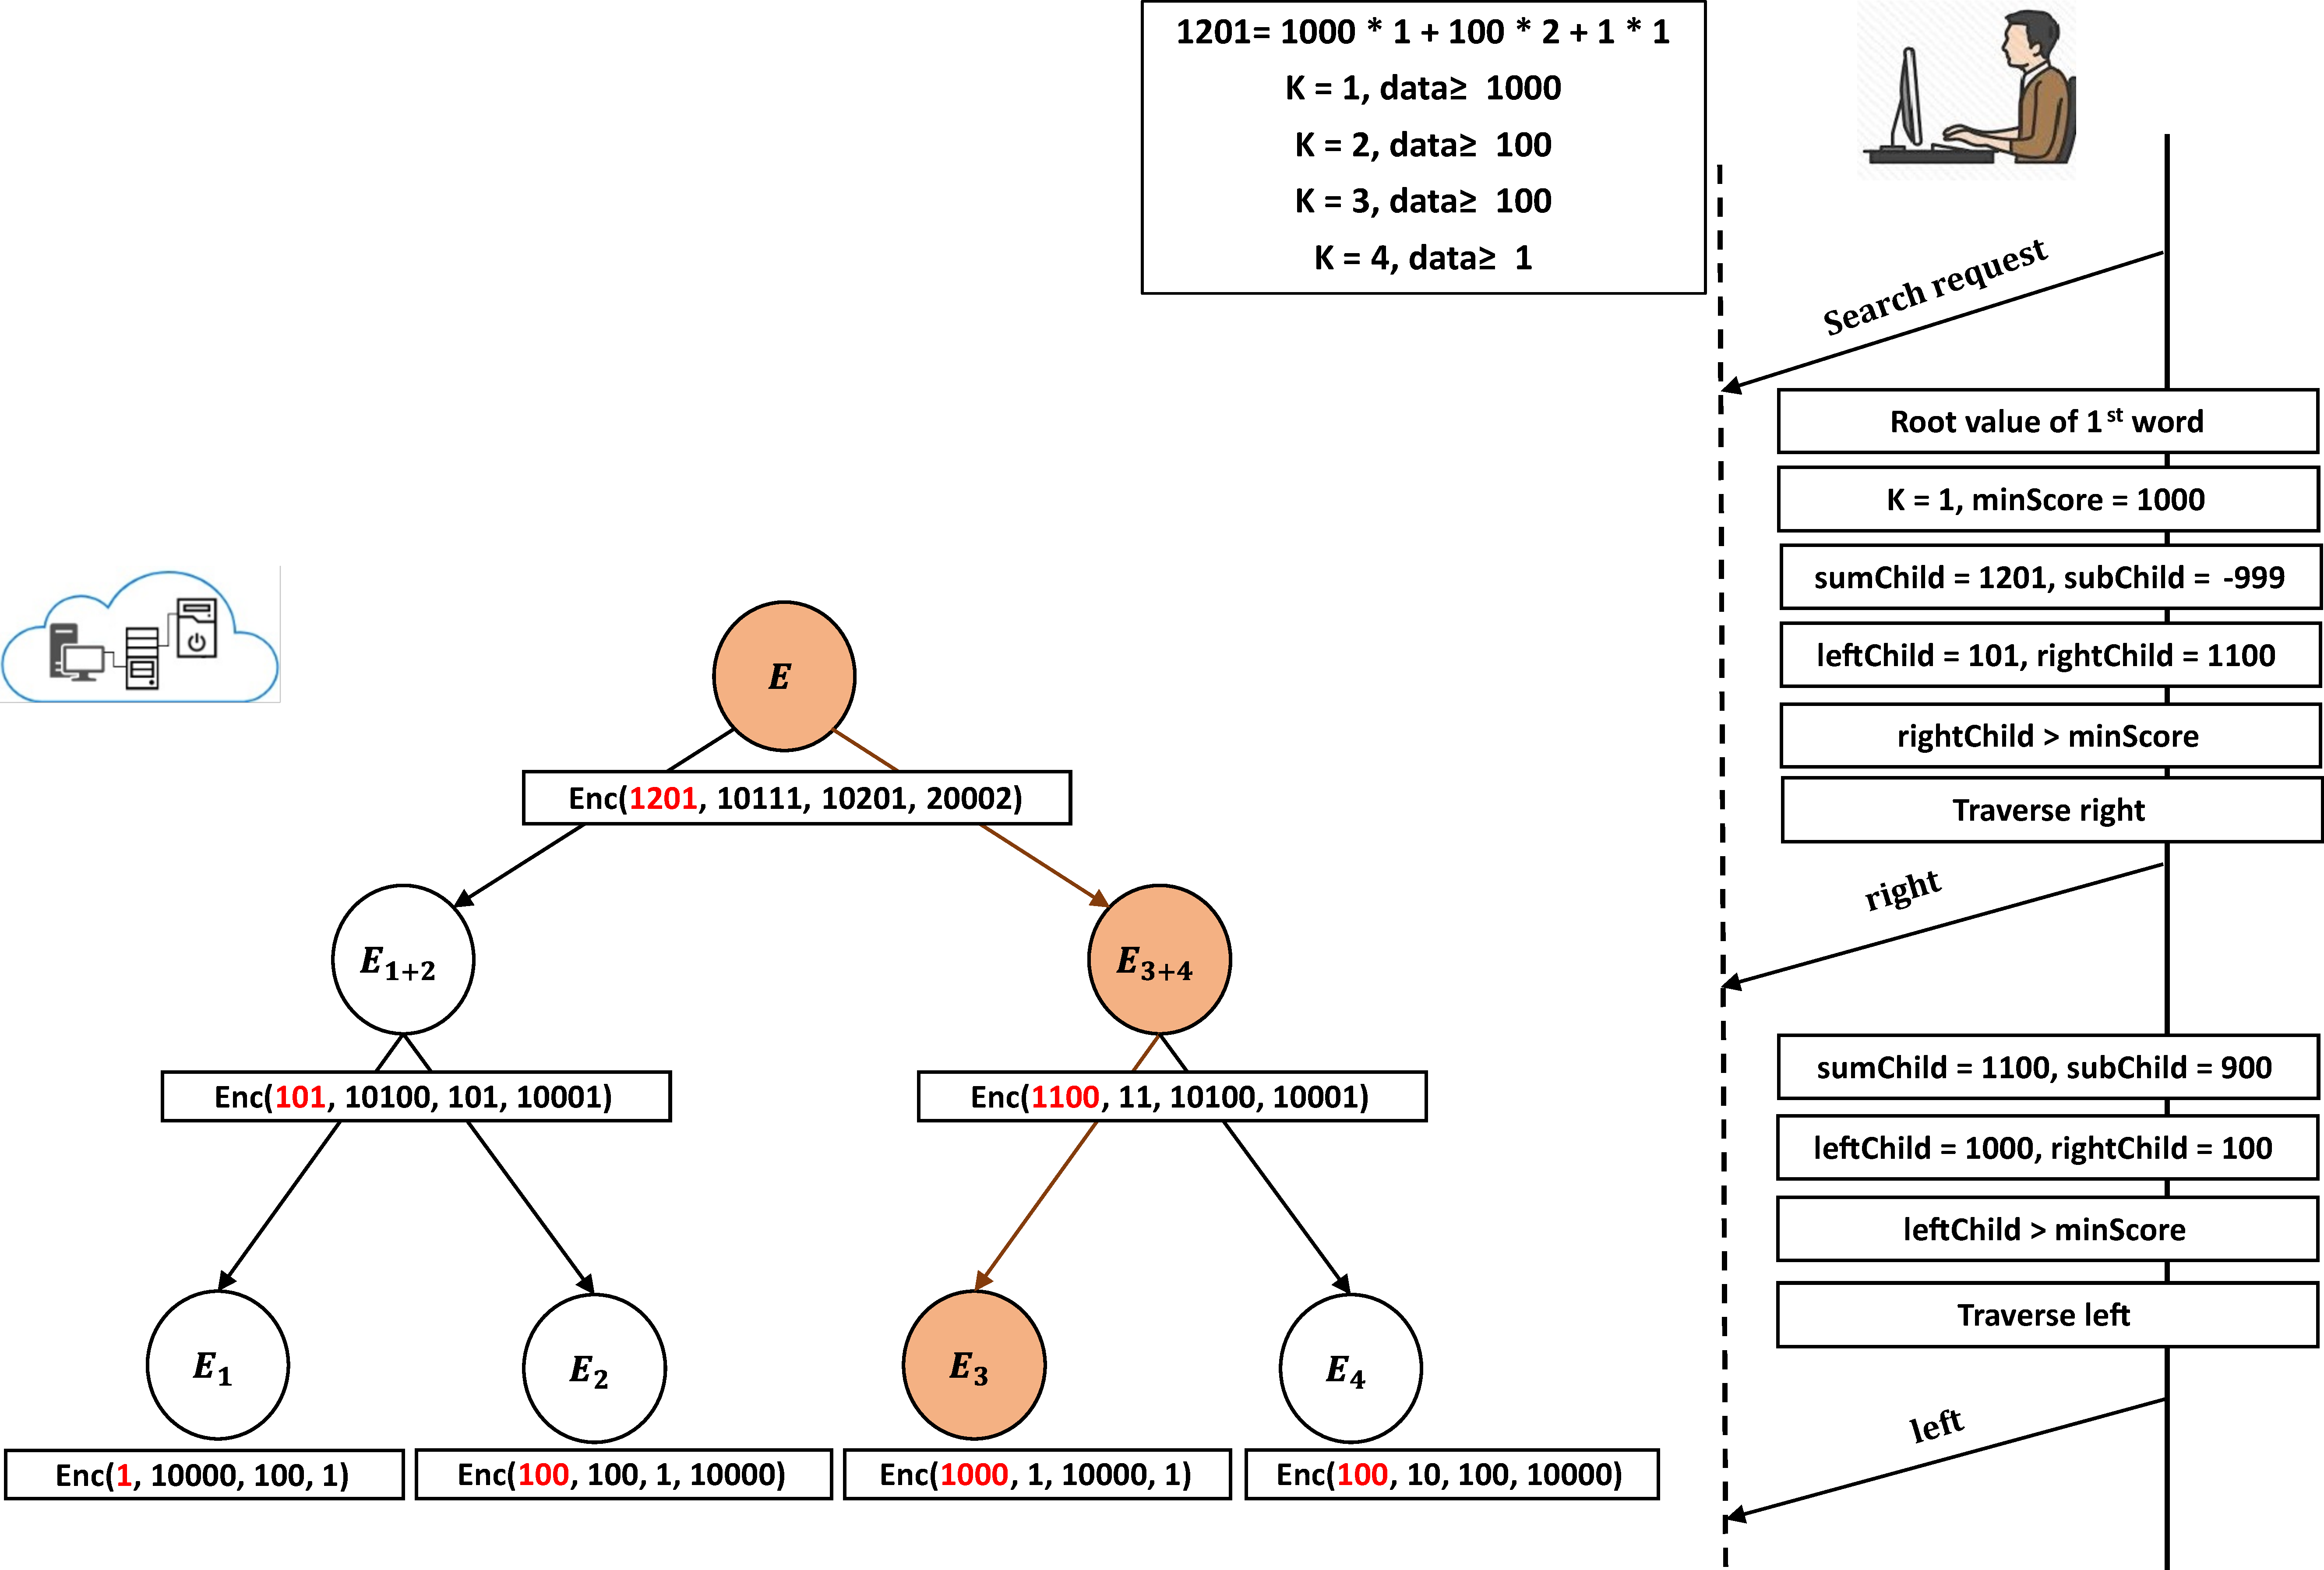
\includegraphics[width=0.95\linewidth]{pdfs/search-user-cloud.pdf}
\caption{An example of the search process that returns the most relevant document for the $1^{st}$ keyword.}


\label{fig:searching}
\centering
\end{figure}

The formal ranked search procedure from the admin side is presented in Algorithm~\ref{algo:searchingInUserRanked}. We construct a result queue denoted as $priorityQueue$, whose element is defined as $(score, id)$. The $priority-Queue$ stores the $id$ of the $k$ accessed documents with the largest relevance scores $score$ to the query. The elements of the $priority-Queue$ are ranked in descending order according to the $score$. It is updated during the search procedure.


%  Here, the $score$ is the decrypted relevance score ($i^{th}$ value of document index) for the document with $id$.

% From the tree construction process, we can see that the root's $i^{th}$ value is the summation of all leaf nodes $i^{th}$ value, which are various powers of $M$. That means we can find the relevance scores of all leaf nodes from the root node. Therefore, we can compute $minScore$, the minimum relevance score among the $k$ documents, before running the DFS procedure just from the root node.  By converting the root's value into a $M$ base number and taking the highest significant digits until the sum is greater or equal to $k$, then the $minScore$ is $M$\textsuperscript{\textit{number of digits left}}. The DFS need not traverse the nodes which contain the relevance score less than $minScore$, and thus only parts of the tree nodes are accessed.\looseness=-1



% The ranked search procedure starts by the admin taking the root node's value from the cloud and calculating the $minScore$ for top-k ranked documents. Then, the admin calculates the next node to be traversed after the root node. The admin can calculate the values of the child nodes without accessing those nodes. We know that the root node is the summation of its child nodes. Furthermore, the admin can obtain the subtraction vector of a node's child nodes from the cloud. The summation and subtraction of two nodes can be used to find the child nodes' values. These nodes are accessed if these values are higher than $minScore$. This process goes on recursively until the whole tree is covered.\looseness=-1





The admin starts the ranked search procedure taking the root node's value from the cloud and calculating the $minScore$, the minimum relevance score for top-k ranked documents. The DFS need not traverse the nodes which contain the relevance score less than $minScore$, and thus only parts of the tree nodes are accessed. From the tree construction process, we can see that the root's $i^{th}$ value is the summation of all leaf nodes $i^{th}$ value, which are various powers of $M$. That means, we can compute $minScore$ just from the root node. By converting the root's value into a $M$ base number and taking the highest significant digits until the sum is greater or equal to $k$, then the $minScore$ is $M$\textsuperscript{\textit{number of digits left}}. From Fig. ~\ref{fig:searching} we can see that, at first the admin requests the value of the root node from the cloud. After that, the admin converts the root node's $1^{st}$ value (the search is for $1^{st}$ keyword) 1201 into a M (10) base number. 1201 can be written uniquely as 1000*1+ 100*2+10*0+1*1. We can see from 1000*1+ 100*2+10*0+1*1 that the tree contains one node containing value 1000, two nodes containing value 100, and one node of value 1. Hence, if k=1, data values less than 1000 need not be traversed, if k=2, values less than 100 need not be traversed and so on.\looseness=-1


Then, the admin calculates the next node to be traversed after the root node. The admin can calculate the values of the child nodes without accessing those nodes. In RS-PKE, the internal nodes are the summation of their child nodes and the admin can obtain the subtraction of the child nodes from the cloud. The summation and subtraction of two nodes can be used to find the child nodes' values. These nodes are accessed if these values are higher than $minScore$. This process goes on recursively until the whole tree is covered.\looseness=-1

Fig. ~\ref{fig:searching} shows an example of ranked search where admin searches for $k=1$ document for the $1^{st}$ keyword. The admin first computes $minScore = 1000$. For root node $E$, $sumChild = 1201$ is the summation of its child nodes and the admin gets the subtraction $subChild = -999$ from the cloud. Then admin calculates left child's value $(sumChild+subChild)/2=101$ and the right child's value $(sumChild-subChild)/2=1100$. As only $E_{(3+4)}$ has values greater than 1000, therefore, only the left node is traversed after root node. This process goes on and finally leaf node $E_{3}$ is the search result. The admin takes the document that corresponds to $E_{3}$ from the cloud.\looseness=-1


One thing worth mentioning in this search mechanism, it is assumed that the partial homomorphic encryption technique used here supports addition as well as subtraction. If homomorphic subtraction is not supported, both the child nodes of a specific parent node are sent to the admin. The admin then decrypts the vector's value that corresponds to the specific keyword from both the child nodes. These values are then subtracted from one another to decide the next node to be traversed in the index tree.

In the search procedures, all intermediate information is kept on the admin side. The cloud only returns the node's data or homomorphic subtraction of data. Therefore, the cloud can serve multiple search requests in parallel. 



\subsection{Leakage}\label{leakage}

RS-PKE reveals some information to the cloud server for efficiency, like all other practical SE schemes. The leakage of our scheme $\mathcal{L}_{RS-PKE}$ can occur in three phases, \texttt{Setup}, \texttt{BuildIndexTree}, and \texttt{Search}. We have discussed the leakages of our construction below:


$\mathcal{L}_{Setup}$. The cloud performs partial homomorphic addition to generate the KBB index tree. Therefore, the cloud needs to know some parameters from the generated keys to perform the addition. Depending on the PHE chosen, the information can vary, though in most cases, this reveals the highest value, $hValue$ that can be encrypted with the generated public key. In RS-PKE, the highest value to be encoded for a specific keyword in the dictionary is $M^\alpha$. For performance, $hValue$ is close to $M^\alpha$. The cloud can estimate $M^\alpha$ from $hValue$. Therefore, $\mathcal{L}_{Setup} = (M^\alpha)$.


$\mathcal{L}_{BuildIndexTree}$. During the \texttt{BuildIndexTree}, the cloud receives the encrypted document $c$, document index and generates an id for the document. The cloud learns the size of $c$ and dictionary size $N$ (by observing the number of entries in the document index). Therefore, $\mathcal{L}_{BuildIndexTree} = (N, |c|, id)$.


$\mathcal{L}_{Search}$. During the interactive \texttt{Search} procedure between the cloud and the admin, the cloud can keep track of the search path through the KBB tree. The resulting documents for a queried keyword are retrieved by their ids from the cloud. Keeping track of the search path is not a leakage as if given $k$ ids, the search path can be reconstructed because the path to any id from the root is unique. The only leakage is the response ids, which is also called the access pattern \cite{Islam2012AccessPD}. The leakage of access pattern in RS-PKE implies that for same document collection, for same keyword, same ids are returned as a search result. Therefore, $\mathcal{L}_{Search} = (id_1, id_2, id_3,\dots,id_k)$.

 

\subsection{Security Analysis}\label{sec-prof}


In RS-PKE, the documents themselves can be encrypted with any standard file encryption technique. The security analysis of these standard encryption techniques is out of the scope of this research. Our goal is to prove the security models defined in Section~\ref{security-model} against an ``honest but curious'' cloud server.




\textbf{IND-SPKE-CKA}: The formal security claim of the IND-SPKE-CKA game, defined in Definition~\ref{ind-spke-cka-game}, is given in Theorem~\ref{ind-spke-cka-prof}.



\begin{theorem}\label{ind-spke-cka-prof}
If a probabilistic polynomial time (PPT) adversary $\mathcal{A}$ can break the \textbf{IND-SPKE-CKA} security of our scheme, there is a PPT adversary $\mathcal{B}$ who can break the \textbf{IND-CCA1} security of underlying PHE.
\end{theorem}

 
IND-SPKE-CKA security of our scheme depends on the IND-CCA1 security of the underlying PHE scheme. The proof is postponed to Appendix~\ref{app-ind-spke-cka-prof}.


\textbf{IND-SPKE-CSKA}: The formal security claim of IND-SPKE-CSKA game, defined in Definition~\ref{IND-SPKE-CSKA-game}, is given in Theorem~\ref{IND-SPKE-CSKA-prof}.




\begin{theorem}\label{IND-SPKE-CSKA-prof}
If a PPT adversary $\mathcal{A}$ can break the \textbf{IND-SPKE-CSKA} security of our scheme, $\mathcal{A}$ can also break the \textbf{IND-SPKE-CKA} security of our scheme.
\end{theorem}

IND-SPKE-CSKA depends on the fact that $\mathcal{L}_{Search}$ is only limited to access pattern, which makes IND-SPKE-CSKA a restricted version of IND-SPKE-CKA. The proof is postponed to Appendix~\ref{app-IND-SPKE-CSKA-prof}.



\textbf{Forward Privacy}: The forward privacy of RS-PKE, defined in Definition~\ref{fs-game}, is proved using Theorem~\ref{fs-prof}.

\begin{theorem}\label{fs-prof}
RS-PKE achieves forward privacy if a PPT adversary $\mathcal{A}$ has a negligible advantage of winning the \textbf{IND-SPKE-CKA} game.
\end{theorem}


IND-SPKE-CKA security of RS-PKE is sufficient to ensure forward privacy. The proof is given to Appendix~\ref{app-fs-prof}.







\section{Performance Evaluation}\label{evaluation}

We have implemented the RS-PKE using Java language. Our entities (document producer, cloud server, and admin) are Java applications (jar) that connect through the REST protocol using Spring Framework. We have used Paillier PHE scheme \cite{Paillier:1999}, to encrypt and decrypt the document indexes generated from document producers. Javallier\footnote{\url{https://github.com/n1analytics/javallier}}, a Java library for Paillier partially homomorphic encryption, is used as our encryption library.\looseness=-1

The efficiency of the system is tested on the Request for Comments (RFC) dataset. The RFC dataset contains almost 8582 plain text documents with a total size of approximately 445 MB. RFC contains technical and organizational documents about the Internet, including the specifications and policy documents \cite{rfc}. It is a widely used dataset in SE literature \cite{wang2010secure, wang2011enabling, smithamol2018pecs, xia2015secure, peng2018efficient}. The dictionary $W$ contains 1000 English words extracted from the RFC dataset. 


For implementing the application in the cloud, we have used Amazon EC2 cloud service's \textit{t3a.xlarge} (AMD EPYC 7000 series 2.5GHz 4 core processor with 32GiB memory) instance as the \textit{cloud server} and \textit{t2.micro} (Intel Xeon 3.3 GHz 1 core processor with 1GiB ram) instance for \textit{admin}. And we took the lowest possible AWS instance \textit{t2.nano} (Intel Xeon 3.3 GHz 1 core processor with 0.5GiB ram) instance for \textit{document producer}. The test includes: (1) the efficiency and storage requirements of single encrypted document index generation, (2) the efficiency and storage requirements of dynamic index construction, and (3) the efficiency and accuracy of the search. We make our implementation open-source\footnote{\url{https://github.com/pkse-searcher/secure-pkse}}.\looseness=-1





\subsection{Encrypted Document Index Generation}


\begin{figure}[htpb]
    \centering
    \subfloat[]{
       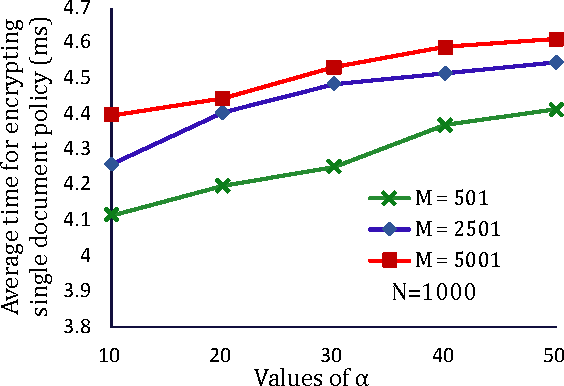
\includegraphics[width=0.45\linewidth]{avgTimeEncryption}}
    \hfill
  \subfloat[]{
        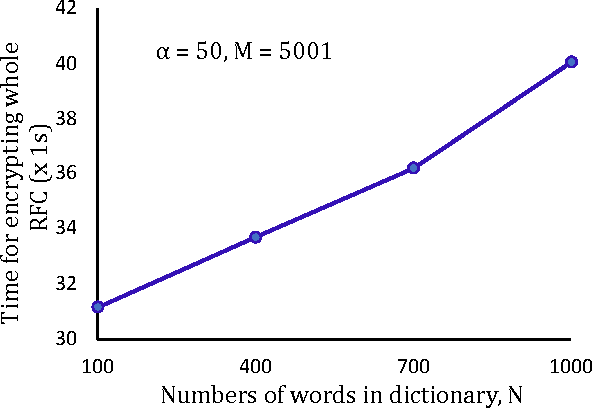
\includegraphics[width=0.45\linewidth]{avgTimeEncryption2}}
 
    \subfloat[]{
       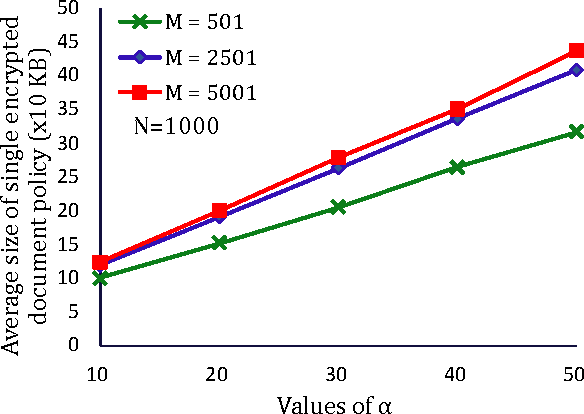
\includegraphics[width=0.45\linewidth]{avgSizeEncryption}}
    \hfill
  \subfloat[]{
        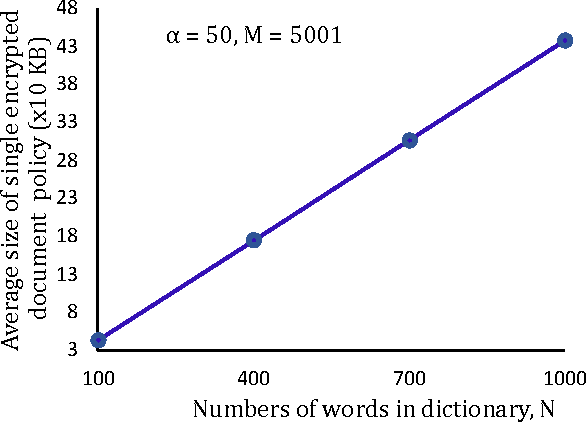
\includegraphics[width=0.45\linewidth]{avgSizeEncryption2}}
  \caption{\small{Average time cost for generating encrypted single document index (a) \& (b) and average size cost for encrypted single document index (c) \& (d).}}
  \label{fig:avgSizeEncryption} 
\end{figure}



The encrypted document index generation process includes two main steps: 

\begin{enumerate}
    \item \textit{Construction of normalized vector}: The largest value for the normalized vector for a specific keyword in the dictionary is $M^\alpha$.
    
    \item \textit{Encrypting the normalized vector with the public key of Pailliers PHE}: The size of ($PubKey$, $PrvKey$) pair depends on the value of $\alpha \log{M}$, minimum bits needed to encode $M^\alpha$. For different combinations of $M$ and $\alpha$, the ciphertext size of Paillier is in the range of 144-704 bits.\looseness=-1
\end{enumerate}

There is an encrypted value for each keyword in the dictionary in the document index. Hence, the size complexity of encrypted document index is $O(N \alpha \log{M})$. The time cost for encrypting a single document index is proportional to the single encrypted document index's size. Fig. \ref{fig:avgSizeEncryption} shows how the average time for creating an encrypted document index and the average size of encrypted document index changes with different parameters.





\subsection{Index Tree Construction}


\begin{figure}[htpb]
    
    \subfloat[]{
       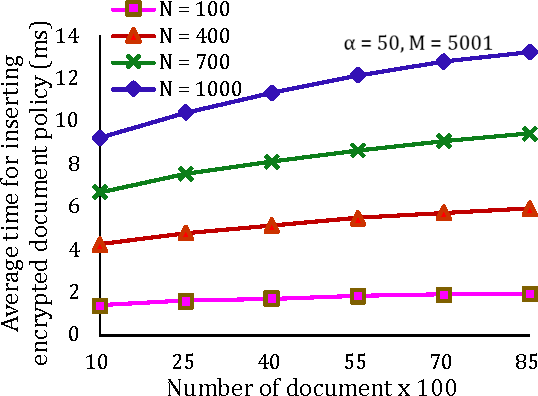
\includegraphics[width=0.45\linewidth]{avgTimeInsert}}
        \hfill
  \subfloat[]{
        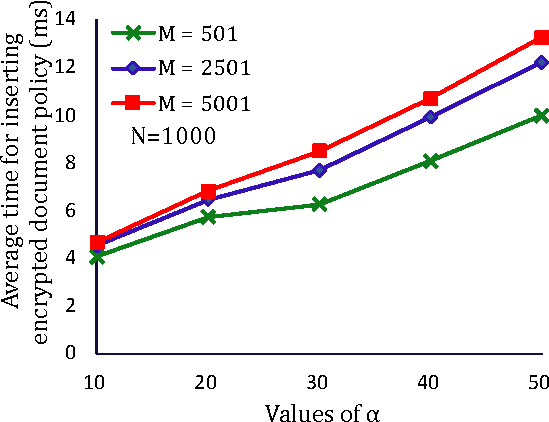
\includegraphics[width=0.45\linewidth]{avgTimeInsert2}}
        
        
        
  \caption{\small{The average time cost for inserting a node in the tree. For (b) the collection of document is fixed, $|F|= 8582$.}}
  \label{fig:tree-insert} 
\end{figure}



The time cost of index tree construction depends on:
\begin{enumerate}
    \item \textit{Number of documents}: The height of the tree expands as the number of documents increases. The insertion of a document as a leaf node only requires the subsequent parent nodes to be updated; therefore, only a single node is accessed at a level. Consequently, time changes logarithmically with the insertion of documents.\looseness=-1
    
    \item \textit{Size of an encrypted document index}: When a leaf node is inserted, a partial homomorphic addition is performed for each element in the document index to update a parent node. The performance of the addition is dependent on the size (number of bits) of the elements. Therefore, the time of inserting a single document index is proportional to $N\alpha \log{M}$.
\end{enumerate}

 As the insertion and deletion operation is almost similar in the sense that insertion involves addition and deletion involves subtraction of encrypted values; therefore, the time complexity is also similar. The time complexity of generating index tree and deleting a node from the index tree is $O( \log{|F|} N \alpha \log{M})$. Fig.~\ref{fig:tree-insert} shows the insertion time. The graphs of deletion are moved to Appendix~\ref{fig:deletion}.
 
 \begin{figure}[htpb]
        
        \subfloat[]{
       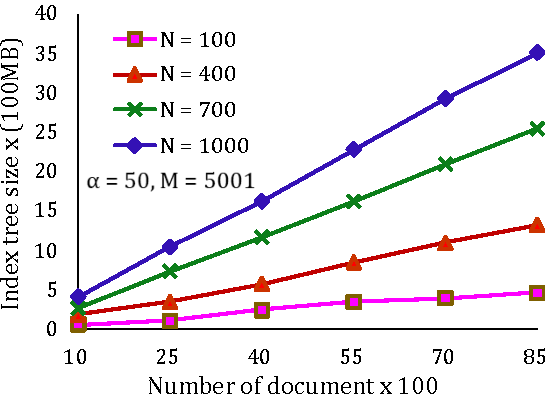
\includegraphics[width=0.45\linewidth]{IndexSize.pdf}}
    \hfill
  \subfloat[]{
        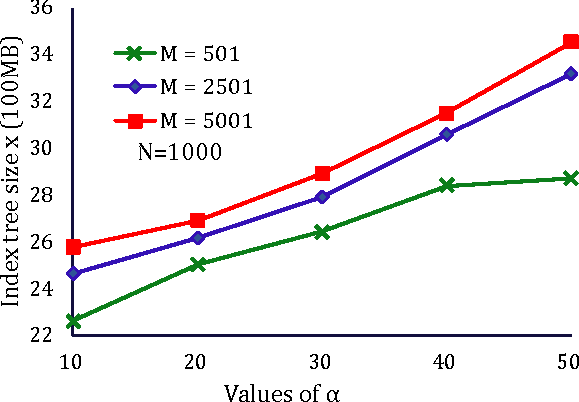
\includegraphics[width=0.45\linewidth]{IndexSize2.pdf}}
  \caption{\small{(a) \& (b) is the size of the KBB tree. For (b) the collection of document is fixed, $F= 8582$.}}
  \label{fig:tree-size} 
\end{figure}

 
 On the other hand, the storage consumption of the index tree is determined by the size of the document collection, $|F|$. Specifically for $|F|$, the number of nodes in the KBB tree is $2|F|-1$. In the KBB tree, every node stores a single encrypted document index, and the document index size is proportional to $N \alpha log(M)$. Therefore, the storage requirement of index tree is $O(|F| N \alpha  \log{M})$. Fig.~\ref{fig:tree-size} shows the size of index tree with different parameters. From the graphs we can see that the storage consumption of the index tree is high. However, that is not a problem as storage is cheap in the cloud.



\subsection{Search Efficiency}


The time complexity of search mainly depends on:

\begin{enumerate}
    \item \textit{The height of the tree}: The height of the tree is $O( \log{|F|} )$. Therefore, the number of documents in the dataset has a small impact on the search.
    
    \item \textit{Network load}: The network load is proportional to the size of an encrypted document index, which is $O(N \alpha \log{M})$.
    
\end{enumerate} 

 For the ranked search, the single ranked search's procedure is repeated $k$ times. Therefore, complexity and network overload change accordingly. Fig. \ref{fig:ranked} shows the time cost of searching that returns a single document and $k$ ranked documents with different parameters, respectively. 



\begin{figure}[!t]
    \centering
    \subfloat[]{
       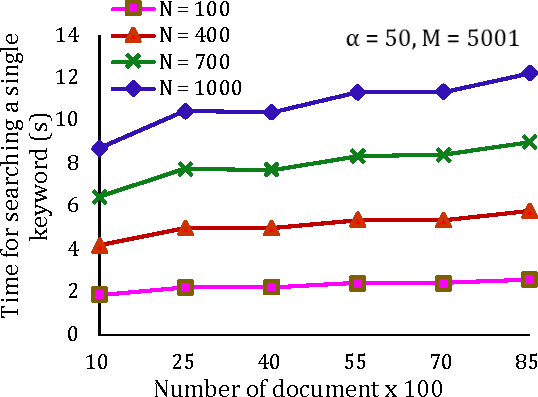
\includegraphics[width=0.45\linewidth]{searchTime.pdf}}
    \hfill
  \subfloat[]{
        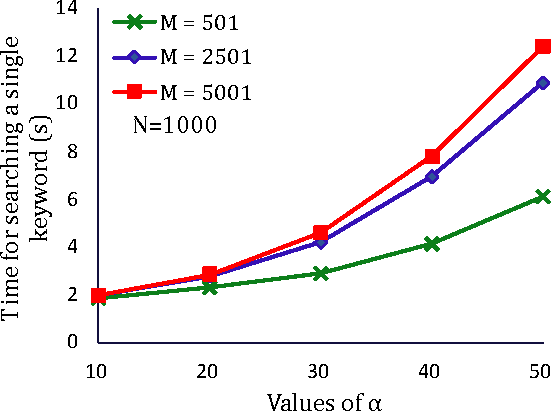
\includegraphics[width=0.45\linewidth]{searchTime2.pdf}}


    \subfloat[]{
       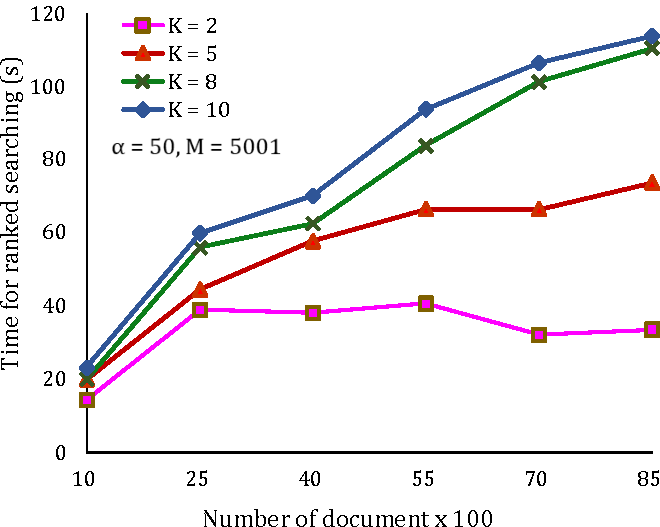
\includegraphics[width=0.45\linewidth]{pdfs/ranked-old.pdf}}
    \hfill
  \subfloat[]{
        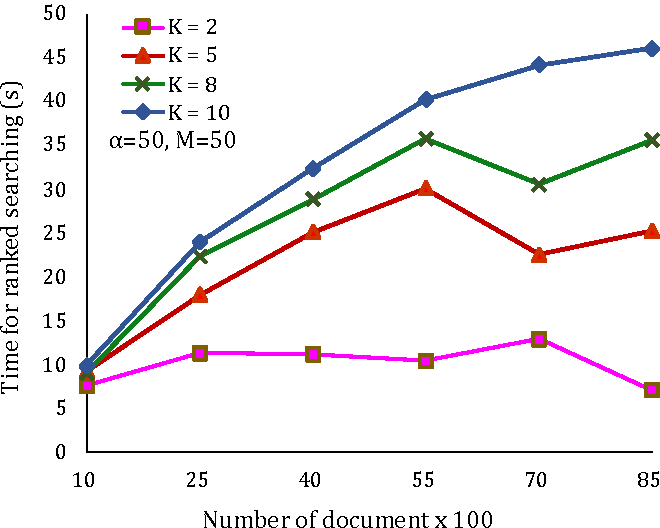
\includegraphics[width=0.45\linewidth]{pdfs/ranked new.pdf}}
  \caption{\small{Average time cost for searching: single document (a) \& (b) and k ranked documents (c) \& (d). For (b) the collection of document is fixed, $F= 8582$.}}
  \label{fig:ranked}
\end{figure}



\subsection{Search Accuracy}

The search precision is defined by the rate of deviation in fetching correct documents for a specific keyword. In Theorem~\ref{b-theorem} we show that, the minimum value of $M$ must be $\lfloor\frac{D_{max}}{2}\rfloor+1$ to get accurate search result. For $M$, a value much smaller than the minimum value can be used in a practical scenario as in the real dataset, the keywords are more distributed. Fig. \ref{error} illustrates that search precision is not affected by values of $M$; different values of $M$ always return the same document. However, precision is greatly affected by the value of $\alpha$. Therefore, care must be taken while choosing the value of $\alpha$ as a smaller value of $\alpha$ can make two slightly different values of $TF$ score normalized to the same value and thus returns incorrect results to a top-k query. Between Fig.~\ref{fig:ranked} (c) and (d), we can see that decreasing $M$ to 10\% decrease the search time to 25-30\%.

\begin{figure}
    \centering
       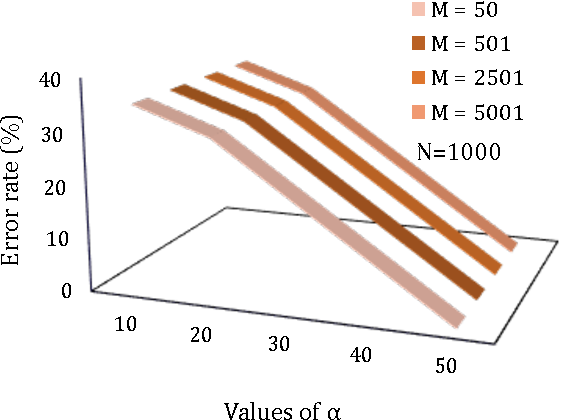
\includegraphics[width=0.6\linewidth]{pdfs/searchAccuracy.pdf}
  \caption{\small{A 3D graph representing the error rate in search results for different $\alpha$ and $M$ with fixed documents and dictionary, $N=1000$.}}
  \label{error} 
\end{figure}

\subsection{Performance Comparison}



We compare the performance of RS-PKE with Xia et al.\cite{xia2015secure}, and Peng et al.\cite{peng2018efficient}. We are comparing our scheme with two SSE schemes instead of other IoT supported SPKE because no other IoT supported SPKE supports top-k ranked search. Xia et al.'s scheme is not efficient for IoT as the number of tree nodes are fixed. The tree is generated initially with all the documents. For dynamic new document insertion, the tree needs to delete an old document and then insert the new one in its place. In Fig.~\ref{fig:comparisonFig}(b), we show comparison of both initially generating tree with all documents and regenerating the tree with dynamic updates. The dynamic update graph of Xia et al. is more comparable with RS-PKE as all our tree operations are dynamic. Xia et al. also requires the owner to perform on the unencrypted index tree to generate the update. Storing the index tree in IoT's end and updating it is not feasible for IoT devices. From Fig.~\ref{fig:comparisonFig}, we can see that Xia et al.'s \cite{xia2015secure} scheme performs better in search, whereas RS-PKE is better at generating the tree with dynamic updates. RS-PKE also does not need the document producers to store any details. Peng et al.'s \cite{peng2018efficient} scheme is not efficient like Xia et al. as this scheme supports the multi-owner with different keys, and each data owner creates an index tree in his part, which is then merged in the cloud. However, they do not support dynamic updates from the same user. SSE schemes are fast due to their faster symmetric-key encryption; however, they are not suitable for lightweight platforms for the risk of key leakage. The mentioned schemes also do not support forward security. Our goal is to make an SPKE for IoT, which will support top-k ranked search with forwarding security without being impractically slow. We think RS-PKE is on the right path for implementing SE in the cloud on encrypted data from lightweight platforms.\looseness=-1


\begin{figure}
    \centering
    \subfloat[]{
       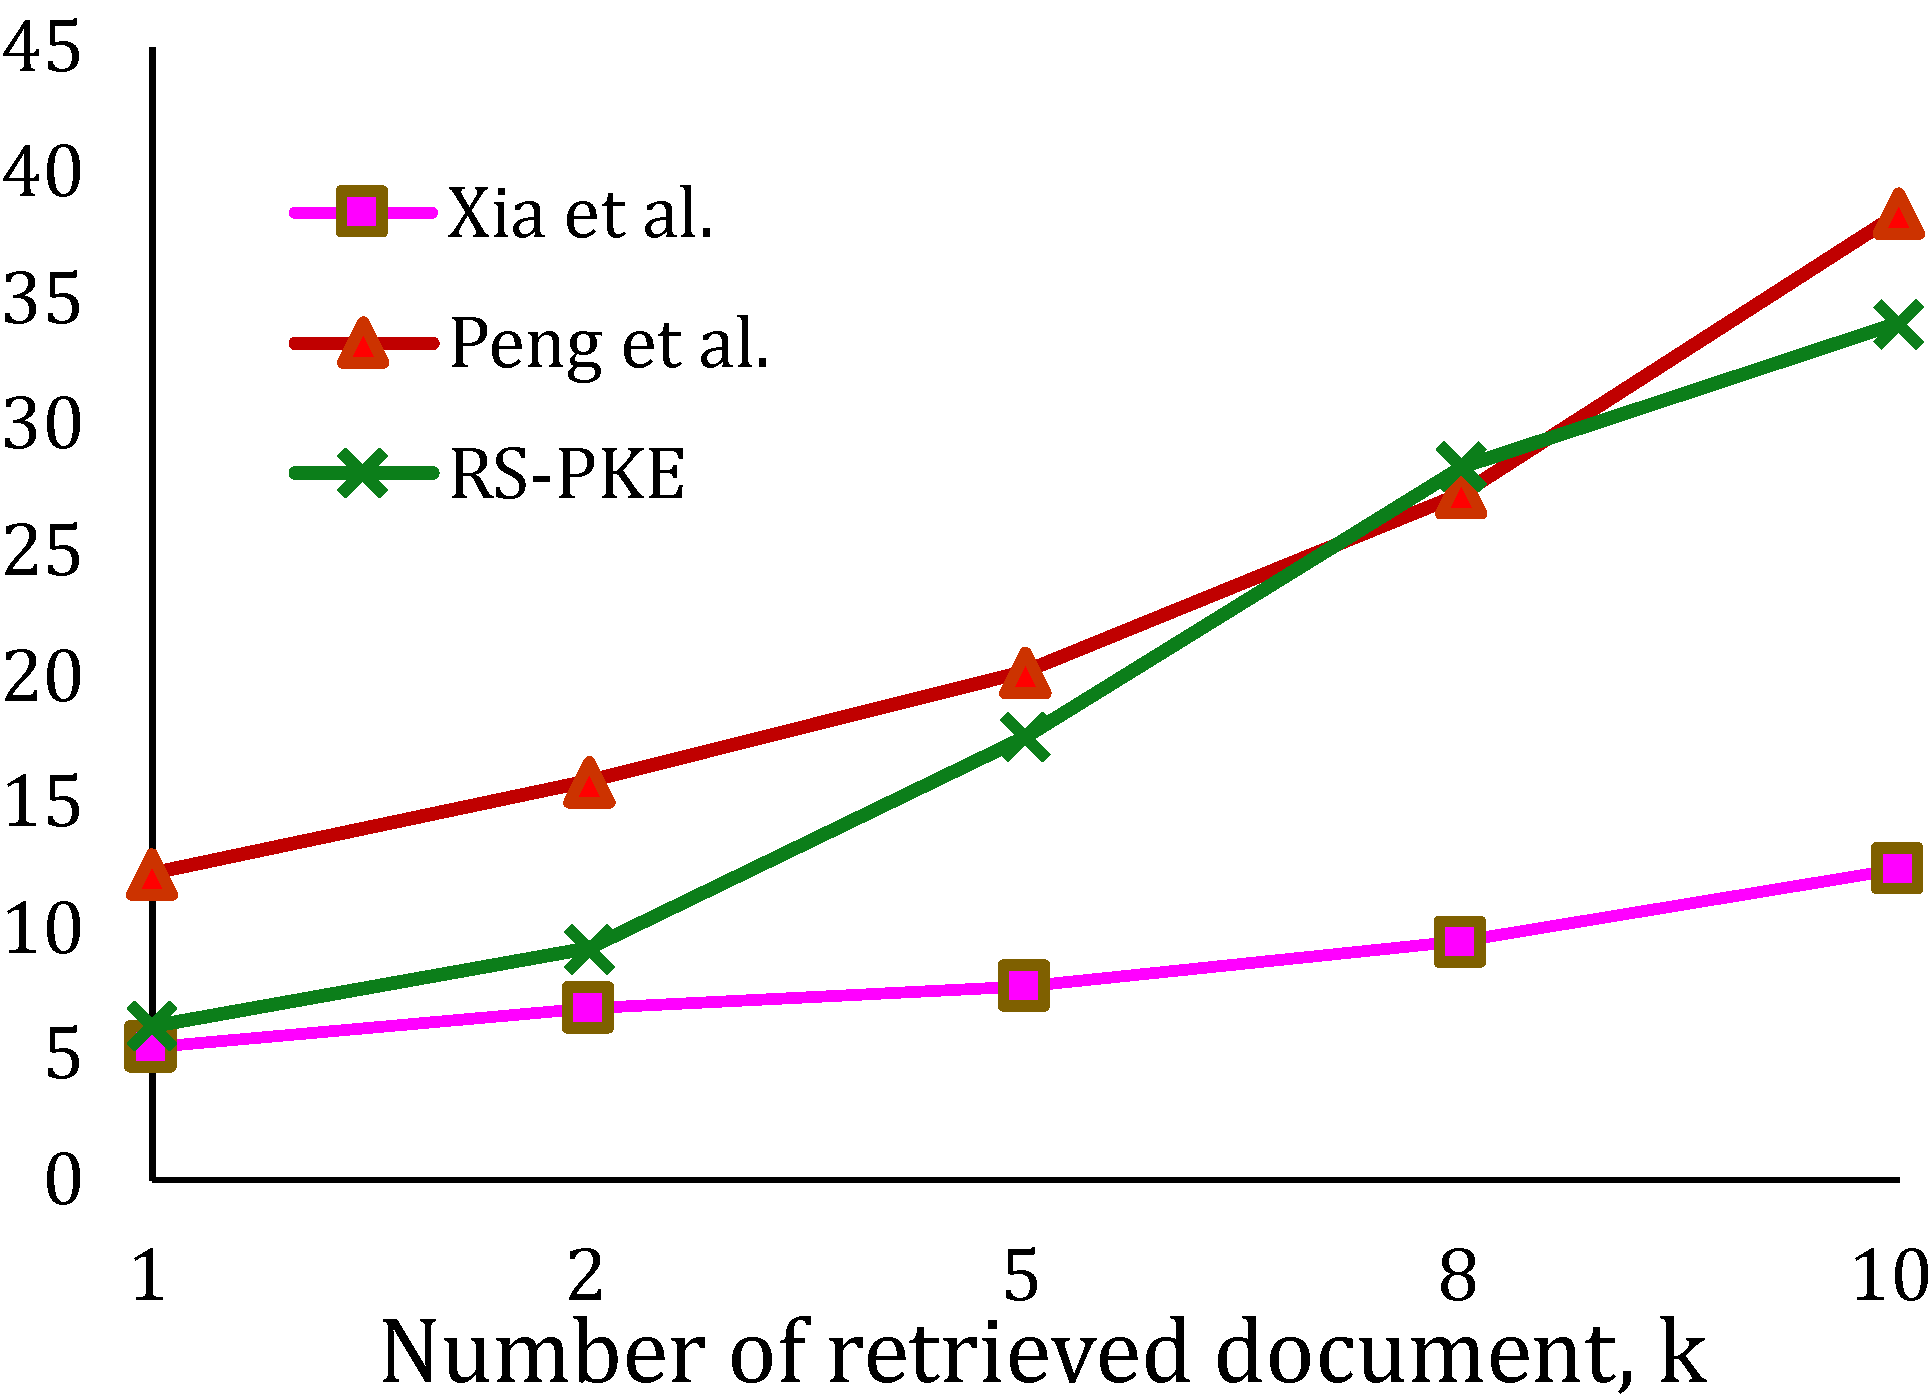
\includegraphics[width=0.45\linewidth]{pdfs/CompareSearch.pdf}}
    \hfill
  \subfloat[]{
        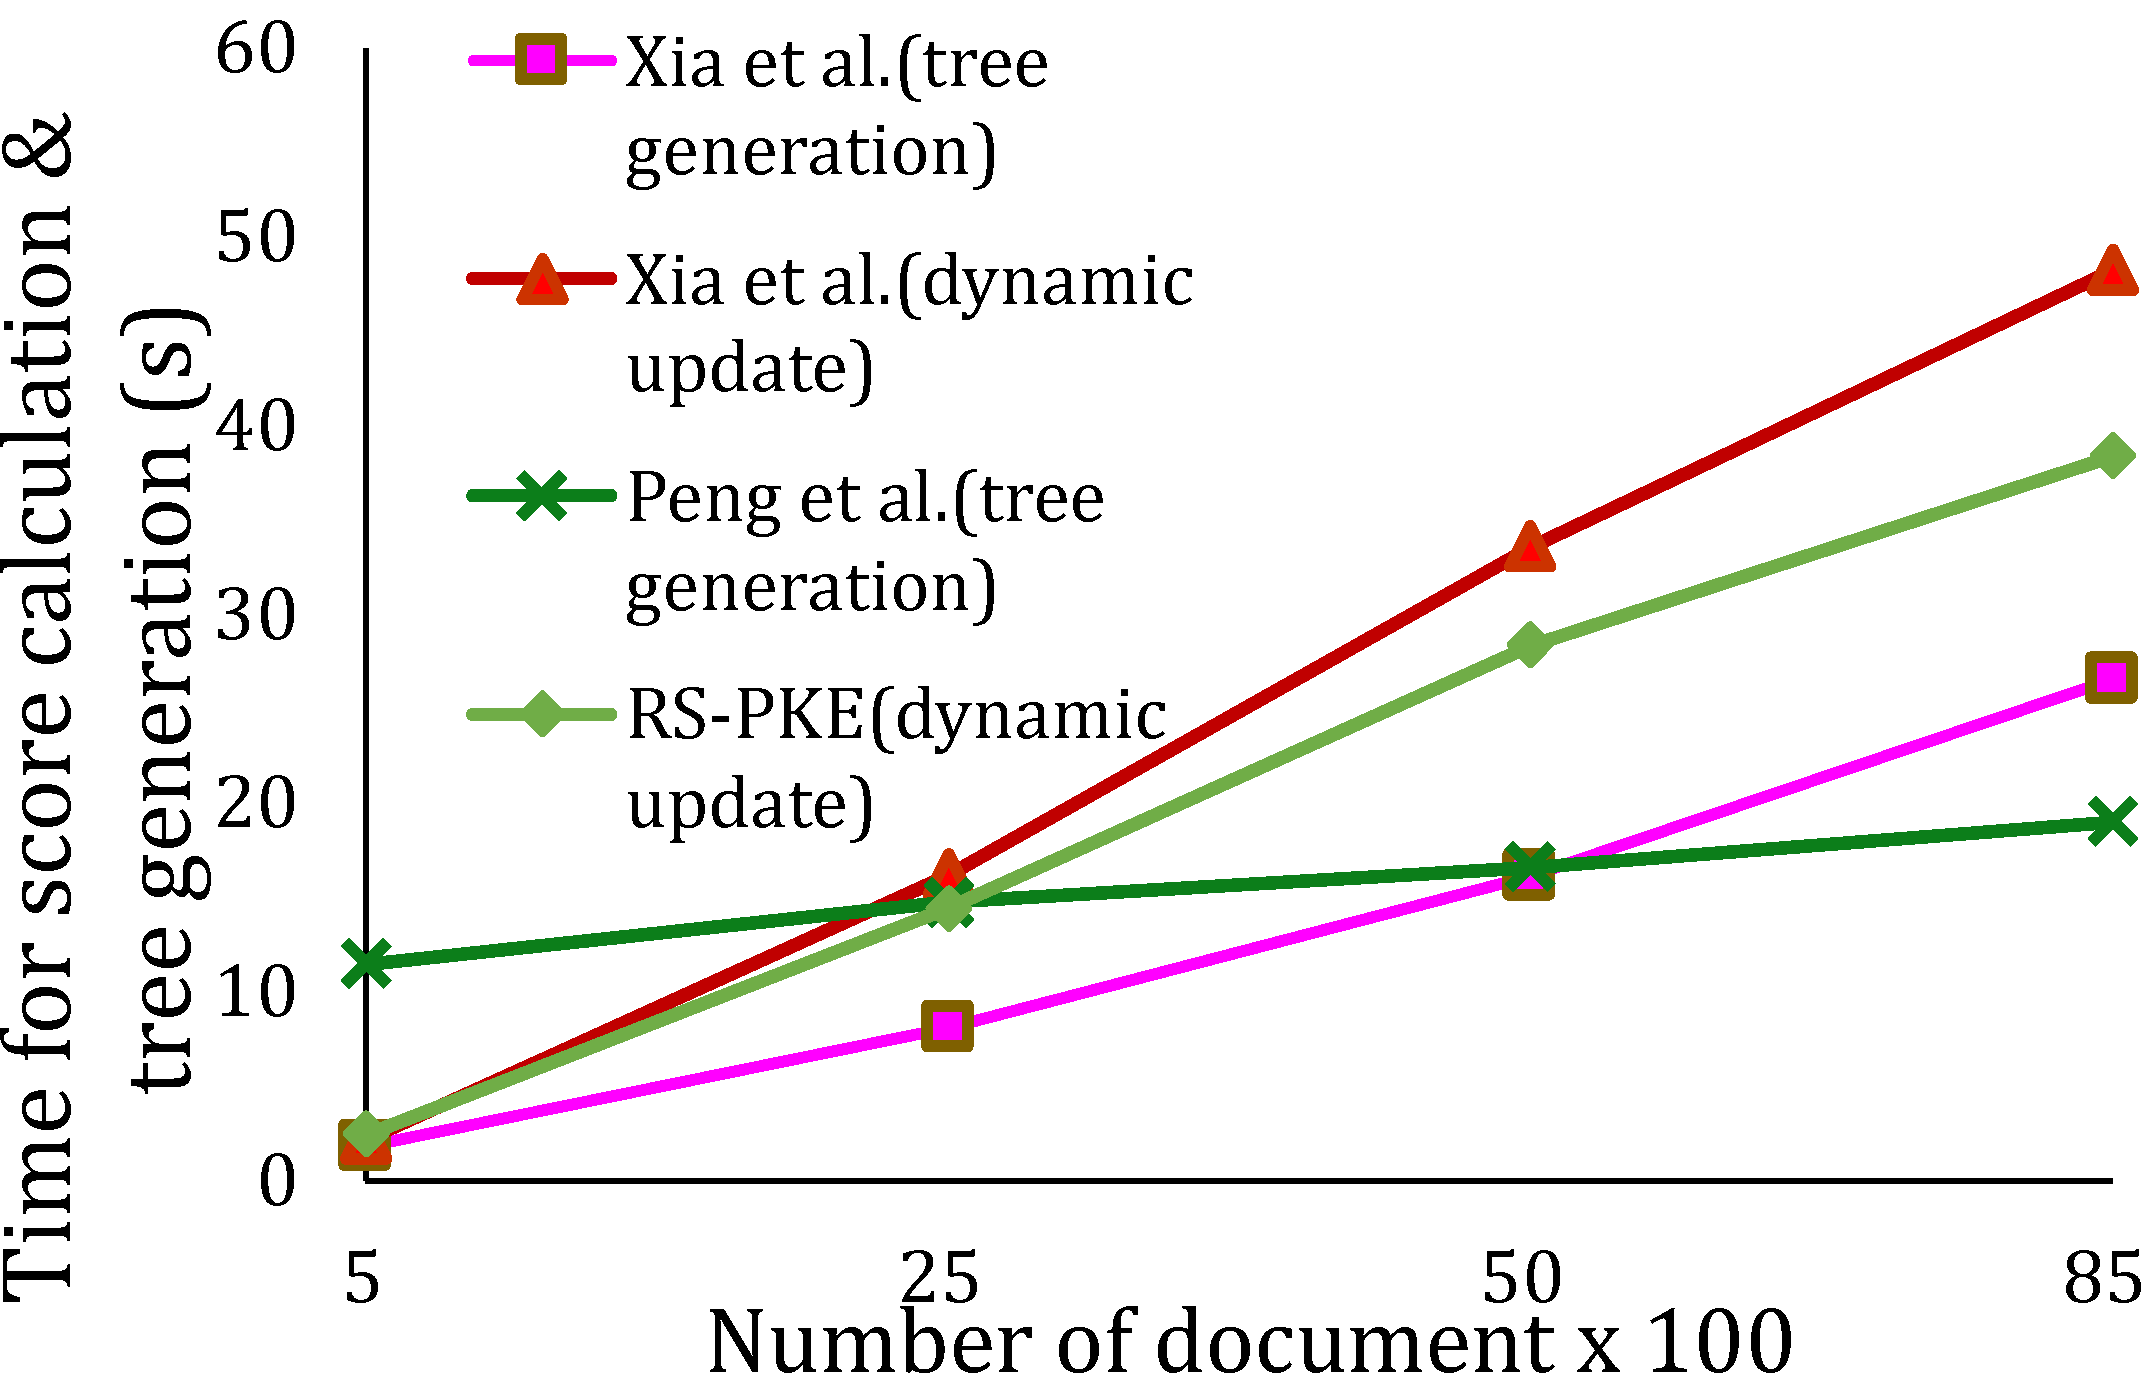
\includegraphics[width=0.45\linewidth]{pdfs/CompareScore.pdf}}
  \caption{\small{Average time for (a) single keyword search for different $k$ and (b) score calculation \& tree generation for different $F$ in different ranked search schemes.}}
  \label{fig:comparisonFig}
\end{figure}







\section{Conclusions}\label{conclusion}
This paper proposes a secure, forward private, efficient, and dynamic SPKE search framework over encrypted cloud data that supports single-keyword ranked search. We analyze the security of encrypted document indexes, KBB based index tree, and search keywords. We have implemented our system in the Amazon EC2 cloud, and extensive experimental results demonstrate our solution's efficiency and scalability.\looseness=-1

The scope of future research includes support of multi-user authentication using different private keys, and efficient multi-keyword ranked search with the \textit{TF-IDF} model. In addition, RS-PKE's encrypted KBB tree's path traversal during search has similarities with private decision tree evaluation. Therefore, further research can be done to use private decision tree evaluation techniques like \cite{kiss2019sok} in RS-PKE to increase efficiency.\looseness=-1


Our scheme mainly considers the security challenges associated with an ``honest but curious'' cloud server, but privacy under a malicious cloud server should also be researched. Especially under a malicious cloud,  backward privacy is required to resist leakage abuse attacks. Furthermore, some of the lightweight devices will likely be malicious in a distributed network for their diversity. These security issues can be incorporated in future researches.\looseness=-1


%% Paper End



%%
%% The next two lines define the bibliography style to be used, and
%% the bibliography file.
\bibliographystyle{ACM-Reference-Format}
\bibliography{sample-base}

%%
%% If your work has an appendix, this is the place to put it.
\appendix

\section{Indistinguishability under Adaptive Chosen Ciphertext Attack}\label{ind-cca1}

 
 
 The $IND$ notation provides security definitions in terms of games. Here a challenger keeps his key secret but gives some specific capabilities to any adversary, and an adversary, with the help of that capabilities, tries to break the security of the encryption. 
 
 \begin{definition}
  
  \textbf{\textit{Setup}}. The challenger runs the algorithm $KeyGen(\mathcal{P})$) and generates the public-private key pair and gives the public key to the adversary and keeps the private key to itself.
  
  \textbf{\textit{Test query-1}}. The adversary can adaptively request the challenger to call the encryption or decryption oracle for its choice of plaintext/ciphertext as many times as he wants.
  

\textbf{\textit{Challenge}}. The adversary sends the Challenger two distinct chosen plaintexts of the same length $message_0$ and $message_1$ of its choice, which it wishes to be challenged. The challenger picks $b\leftarrow\{0,1\}$ uniformly at random and generates a ciphertext $C_b = Enc(PubKey, message_{b})$. The challenger sends $C_b$ back to the adversary.


\textbf{\textit{Test query-2}}. The adversary can perform additional computations in polynomial time.

\textbf{\textit{Output}}  Finally, the adversary outputs a $guess$ for the value of $b$. If $guess=b$, the adversary wins.


  
 \end{definition}
 
 
 The advantage of a adversary in IND-CCA1 is, 
 $Adv_{adversary}^{IND-CCA1} = Pr[guess = b]-\frac{1}{2}$.
 Any scheme is IND-CCA1 secure if no adversary has a non-negligible advantage in winning the above game.
 
 \section{Proof of Theorem~\ref{b-theorem}}
 \label{b-proof}
 \begin{proof}

For the first property,
\begin{equation} 
b(0) = M^0 = 1
\end{equation}
which is smallest value of $M^s$ where $s$ is non-negative. This proves the first property.
 
For the second property, equation~\ref{eq3_1} can be rewritten as, 
\begin{equation} 
\label{eq3}
 b(s) = M * M^{s-1} 
  = M * b(s-1) 
  > (M-1) * b(s-1) 
\end{equation}

Hence, $b(s) > (M-1) * b(s-1)$ ensures the second property $b(i_{max}) > \sum b(j)$ that if the maximum value leaf node resides on the right subtree of root, the sum of all leaf nodes of the left subtree won’t be greater than the maximum value.\looseness=-1
\end{proof}
 
\section{Security Proofs}

\subsection{Proof of Theorem~\ref{ind-spke-cka-prof}}\label{app-ind-spke-cka-prof}

 
Without loss of generality, let us assume, $\mathcal{A}$ is a subroutine of $\mathcal{B}$ and is transparent to the challenger $\mathcal{C}$. $\mathcal{A}$ is the adversary, and $\mathcal{B}$ is the challenger in the IND-SPKE-CKA game while $\mathcal{B}$ is the adversary and $\mathcal{C}$ is the challenger in the IND-CCA1 game.

\textbf{\textit{Setup:}} $\mathcal{C}$ runs the $KeyGen(\mathcal{P})$ algorithm and gives the $PubKey$ to $\mathcal{B}$ and $\mathcal{B}$ sends the $PubKey$ to $\mathcal{A}$. 

\textbf{\textit{Test query-1:}} 
        \paragraph*{Document index generation/encryption} $\mathcal{A}$ sends document $f$ to $\mathcal{B}$. $\mathcal{B}$ generates the \textit{plaintext document index} vector, encrypts each element from $\mathcal{C}$, combines them to $docIndex$ and send them back to $\mathcal{A}$.
        
        \paragraph*{Search/decryption} $\mathcal{A}$ sends a keyword $w$ to $\mathcal{B}$. $\mathcal{B}$ will perform the search procedure using $\mathcal{C}$ for decryption.

\textbf{\textit{Challenge:}} $\mathcal{A}$ sends two documents $f_0$ and $f_1$ to $\mathcal{B}$. $\mathcal{B}$ generates two \textit{plaintext document index} vectors $v_0$ and $v_1$ for $f_0$ and $f_1$ respectively. For each position $i$, $\mathcal{B}$ sends $v_{0,i}$ and $v_{1,i}$ to $\mathcal{C}$. $\mathcal{C}$ picks a random value of $b\leftarrow\{0, 1\}$ and use the same $b$ throughout the challenge. For all positions, $\mathcal{C}$ sends back $Enc(v_{b,i})$ to $\mathcal{B}$. $\mathcal{B}$ combines them to a $docIndex$ and forwards it to $\mathcal{A}$.


    \textbf{\textit{Test query-2:}} $\mathcal{A}$ can perform additional computations in polynomial time.

 \textbf{\textit{Output:}} $\mathcal{A}$ outputs guess $b'\in \{0,1\}$ and send to $\mathcal{B}$, and $\mathcal{B}$ will output $b'$ as it's guess for $b$.


In the above process, from the view of challenger $\mathcal{C}$, $\mathcal{B}$ is an adversary who tries to break the IND-CCA1 security of the underlying PHE. From the view of $\mathcal{A}$, $\mathcal{B}$ is the challenger in the IND-SPKE-CKA game in our scheme. If $\mathcal{A}$ can break IND-SPKE-CKA, $\mathcal{B}$ can also break IND-CCA1. Therefore, the advantage of $\mathcal{B}$ breaking the IND-CCA1 security of underlying PHE is greater than or equal to $Adv_{A}^{IND-SPKE-CKA}$. Hence, the IND-SPKE-CKA of our scheme depends solely on the security of underlying PHE.\looseness=-1


\subsection{Proof of Theorem~\ref{IND-SPKE-CSKA-prof}}\label{app-IND-SPKE-CSKA-prof}

As shown in Section~\ref{leakage}, the search leakage $\mathcal{L}_{Search}$ of our scheme is only limited to access pattern. Hahn and Kerschbaum \cite{hahn2014searchable} and later others \cite{sun2018practical, kim2017forward} shown that SE schemes can achieve security in terms of indistinguishability with access pattern leakage. Therefore, the search keyword's security depends on the security of the document index, as discussed below.


From the perspective of $\mathcal{A}$, the challenge phases of the IND-SPKE-CSKA game and IND-SPKE-CKA game are similar. In the challenge phase of the IND-SPKE-CKA, $\mathcal{A}$ receives a $docIndex_b$ for a specific document $f_b$, and in the IND-SPKE-CSKA, $\mathcal{A}$ receives a $docIndex_b$, as a search result for a specific keyword $w_b$. The test phases of IND-SPKE-CSKA are a more restricted version of IND-SPKE-CKA. Therefore, $Adv_{\mathcal{A}}^{IND-SPKE-CSKA}$ $\leq$ $Adv_{\mathcal{A}}^{IND-SPKE-CKA}$.



\subsection{Proof of Theorem~\ref{fs-prof}}\label{app-fs-prof}

From the view of $\mathcal{A}$, $\mathcal{A}$ has fewer capabilities in FS-SPKEs' test query-1 and test query-2 phases than IND-SPKE-CKA. Theorem~\ref{ind-spke-cka-prof} proves that $\mathcal{A}$ cannot distinguish between document indexes if the PHE is IND-CCA1 secure. The advantage that $\mathcal{A}$ wins the challenge depends on the security of document indexes. Therefore, $Adv_{\mathcal{A}}^{FS-SPKE} \leq Adv_{\mathcal{A}}^{IND-SPKE-CKA}$.


\newpage
\section{Deletion in Tree}\label{app-TreeDelete}
The performance analysis of the deletion algorithm is given in Fig.~\ref{fig:deletion}.
\begin{figure}[!h]
    \subfloat[]{
       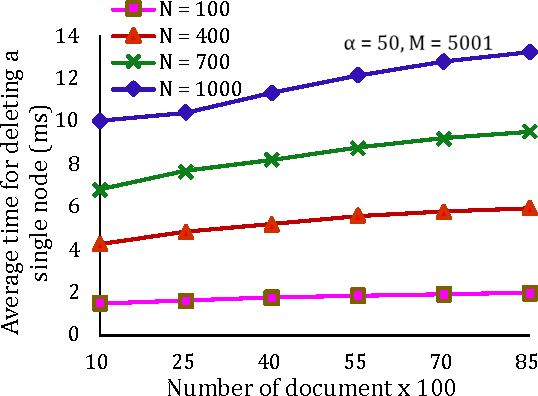
\includegraphics[width=0.45\linewidth]{deletion}}
        \hfill
  \subfloat[]{
        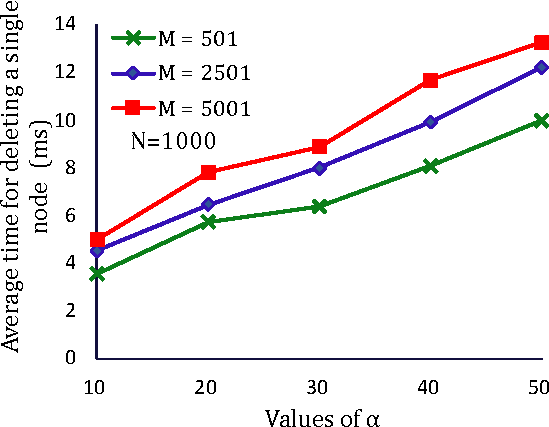
\includegraphics[width=0.45\linewidth]{deletion2}}
    
  \caption{Average time cost for deleting a node. For (b), $F= 8582$ is fixed.}
  \label{fig:deletion} 
\end{figure}



\end{document}
\endinput
%%
%% End of file `sample-sigconf.tex'.
